% book example for classicthesis.sty
\documentclass[
  % Replace twoside with oneside if you are printing your thesis on a single side
  % of the paper, or for viewing on screen.
  oneside,
  %twoside,
  11pt, a4paper,
  footinclude=true,
  headinclude=true,
  cleardoublepage=empty
]{scrbook}

\setlength{\marginparwidth}{2cm}

\usepackage{indentfirst}
\usepackage{dissertation}
\usepackage{float}
%---
\usepackage[T1]{fontenc}
\usepackage{textcomp}
%---
\usepackage[titles]{tocloft}
%% Aesthetic spacing redefines that look nicer to me than the defaults.
\setlength{\cftbeforechapskip}{2ex}
\setlength{\cftbeforesecskip}{0.5ex}
%% Use Helvetica-Narrow Bold for Chapter entries
\renewcommand{\cftpartfont}{%
  \fontsize{12}{14}\usefont{OT1}{phv}{bc}{n}\selectfont
}
\renewcommand{\cftchapfont}{%
  \fontsize{11}{13}\usefont{OT1}{phv}{bc}{n}\selectfont
}
\renewcommand{\cftsecfont}{%
  \fontsize{10}{11}\usefont{OT1}{phv}{}{n}\selectfont
}
\renewcommand{\cftsubsecfont}{%
  \fontsize{9}{10}\usefont{OT1}{phv}{}{n}\selectfont
}
\renewcommand{\cftfigfont}{%
  \fontsize{9}{10}\usefont{OT1}{phv}{}{n}\selectfont
}
\renewcommand{\cfttabfont}{%
  \fontsize{9}{10}\usefont{OT1}{phv}{}{n}\selectfont
}
%---
%usepackage[scaled=.92]{helvet}
\usepackage[all]{xy}
\usepackage{circuitikz}

\titleclass{\subsubsubsection}{straight}[\subsection]


% Title

\titleA{Formalizing ROS2 security configuration with Alloy}

% Author

\author{Luís Mário Macedo Ribeiro}

% Supervisor(es)

\supervisor{Manuel Alcino Pereira da Cunha}

\cosupervisorA{André Filipe Faria dos Santos}

% Date

\date{\myear} % change to text if date is not today

%\makeglossaries %  either use this ...

\makeindex	% ... or this

\begin{document}\fontfamily{phv}\fontseries{mc}\selectfont

% Add acronym definitions

% Cover page ---------------------------------------------
%	\thispagestyle{empty}
	%!TEX root = dissertation.tex

\makeatletter

% UM_ENg Logo
\def\UMEng#1#2{\begin{tikzpicture}[
	% bars styling,
	logone/.style={rectangle,fill=white,rounded corners=0.08cm,minimum width=0.16cm,inner sep=0pt},
	bigone/.style={minimum height=0.74cm},
	smaone/.style={minimum height=0.48cm},
	engone/.style={minimum height=0.86cm},
	pos1/.style={xshift=1.3cm,yshift=1.3cm},
	pos2/.style={xshift=3.9cm,yshift=1.3cm}]
	
% Uminho logo
	\fill[fill=#1] (0,0) -- (2.6,0) -- (2.6,2.6) -- (0,2.6) -- cycle;
	\foreach \i in {1,...,3}{
		\node at (\i*120+30:0.45)[logone,bigone,pos1,rotate=\i*120-60]{};
		\node at (\i*120+90:0.60)[logone,smaone,pos1,rotate=\i*120]{};
	}

% EngUminho logo
	\fill[fill=#2] (2.6,0) -- (5.2,0) -- (5.2,2.6) -- (2.6,2.6) -- cycle;
	\foreach \i in {1,...,5}
		\node at (\i*72-90:0.74)[engone,logone,pos2,rotate=\i*72-90]{};
\end{tikzpicture}}

\def\yyy#1{\fontfamily{phv}\fontseries{mc}\selectfont {\ifnum\hide=1\relax\else#1\fi}}
\def\xxx#1{\fontfamily{phv}\fontseries{mc}\selectfont #1}
\def\zzz#1{\fontfamily{phv}\fontseries{mc}\fontseries{b}\selectfont #1}
\def\kkk#1{\fontfamily{phv}\fontseries{mc}\fontseries{b}\selectfont {\ifnum\hide=1\relax\else#1\fi}}

\long\def\coverEtc{
%Logo
~\vskip-4.1cm\rule{4cm}{0pt}\begin{tabular}{l}
\UMEng\umc{eng}
\\\zzz{Universidade do Minho}\rule{0pt}{1cm}
\\\xxx{}{Escola de Engenharia}
\\\xxx{Departamento de  Informática}
\\\rule{0pt}{4cm}
\\\xxx{{\Large\@author}}
\\\rule{0pt}{1em}
\\\zzz{\Large\@titleA}
\\\zzz{\Large\@titleB}
\\\zzz{\Large\@titleC}
\\\rule{0pt}{5cm}
\\\yyy{\large Master dissertation}
\\\yyy{\large Integrated Master’s in Informatics Engineering}
\\\rule{0pt}{6mm}
\\\yyy{\large Dissertation supervised by}
\\\kkk{\@supervisor}\rule{0pt}{4mm}
\\\kkk{\@cosupervisor}
\\\rule{0pt}{4.2cm}
\\\xxx{{\small\@date}}
\end{tabular}
}


\begin{frontcover}
\gdef\umc{um}\gdef\hide{1}
\thispagestyle{empty} \pagecolor{white} \textcolor{black} \coverEtc
\end{frontcover}

\begin{titlepage}
\gdef\umc{um}
\gdef\hide{0}
\thispagestyle{empty} \pagecolor{white}\textcolor{grey} \coverEtc
\end{titlepage}

\makeatother


%rm
	\cleardoublepage
%---------------------------------------------------------
	\pagenumbering{gobble}
	\setcounter{page}{0}
%---------------------------------------------------------
% Add acknowledgements

\chapter*{Copyright and Terms of Use for Third Party Work}

\noindent This dissertation reports on academic work that can be used by third parties as long as the internationally accepted standards and good practices are respected concerning copyright and related rights.
\vskip 1em
\noindent This work can thereafter be used under the terms established in the license below.
\vskip 1em
\noindent Readers needing authorization conditions not provided for in the indicated licensing should contact the author through the RepositóriUM of the University of Minho.

\section*{License granted to users of this work:}

\CCBY % or replace by one in***************** the list below, cf https://alunos.uminho.pt/PT/estudantes/Formataes/3_Despacho_RT-31_2019_Anexo%203-Informa%c3%a7%c3%a3o-Direitor%20de%20Autor.docx
%---------
%\CBYNCND
%\CCBYNCSA
%\CCBYNC
%\CCBYND
%\CCBYSA


%---------

\chapter*{Acknowledgements}
% Write your acknowledgements here. Do not forget to mention the projects and grants that you have benefited from while doing your research, if any. Ask your supervisor about the specific textual format to use. (Funding agencies are quite strict about this.)

	\cleardoublepage

%---------

\chapter*{Statement of Integrity}

\noindent I hereby declare having conducted this academic work with integrity.
\vskip 1em\noindent
I confirm that I have not used plagiarism or any form of undue use of information or falsification of results along the process leading to its elaboration.
\vskip 1em\noindent
I further declare that I have fully acknowledged the Code of Ethical Conduct of the University of Minho.

%---------

% Uncomment as wished

% Add abstracts (en,pt) -----------------------------------------------------------
\chapter*{Abstract}
	
	Industrial restructuring is becoming highly reliant on automation developments, as they bring more efficient and accurate processes with less associated cost. Consequently, robots are rapidly being deployed in a wide range of scenarios, especially where security is demanded. In such cases, it is critical to employ appropriate procedures to verify both the system's quality and security.

	Following the current growth of cyber-physical system, as well as their usage into various technology domains, the development of software applications is demanding due to the complexity behind the integration of needed services, beyond those provided by the operating system. Hereupon, software middleware is increasingly used, since it offers services that support application development and delivery.

	One of the most popular open-source software platforms for building robotic systems is the Robot Operating System (ROS) \cite{1} middleware, where highly configurable robots are usually built by composing third-party modules. A major factor behind its popularity and widespread adoption is its flexibility and interoperability. One drawback of this flexibility, however, lies in the increased security risks that ROS applications face. The emergence of performance and scalability challenges connected to the ROS middleware standard, in addition to security concerns, prompted the creation of ROS2. 

	Robot Operating System 2 (ROS2), which continues to provide a simple, uniform message passing interface to allow components to communicate with each other, is implemented using the Data Distribution Service (DDS) \cite{3} communication protocol, where security guarantees are ensured by DDS-Security specification. Using DDS-Security, it is possible to configure ROS2 to run with security guarantees using the SROS2 toolset \cite{ros-dds-integration}.
	
	This dissertation proposes a technique, based on the software verification perspective, to automatically verify system-wide properties related to the security configuration of ROS2-based applications. The intended purpose is to model the ROS architecture, as well as the network communication behaviour, in Alloy \cite{alloy-6}, a formal specification language and analysis tool supported by a model-finder over which, system-wide properties are subsequently model-checked.

\paragraph{Keywords} Robotics, ROS, ROS2, DDS, SROS2, Security, Software Verification, Alloy
	\cleardoublepage

\chapter*{Resumo}

	A constante implementação da ideia de automização de processos tem motivado a reestruturação nos mais diversos setores industriais, com o objetivo de aumentar a eficiência e precisão nos processos integrados, e consequentemente, reduzir os custos associados. Além disso, esta ideia impulsiona a integração robótica nos mais amplos domínios tecnológicos, especialmente onde a segurança é exigida. Nestes casos, é fundamental adotar técnicas apropriadas de forma a verificar tanto a qualidade do sistema, como a segurança do mesmo.

	Como resultado do atual crescimento de sistemas ciber-físicos, nomeadamente sistemas robóticos, bem como sua utilização em vários domínios tecnológicos, o desenvolvimento de aplicações é exigente devido à complexidade da integração dos serviços necessários, tipicamente não fornecidos pelo sistema operativo. De forma a acompanhar o aumento da complexidade destes sistemas, \textit{middlewares} têm sido adoptados, pois integram serviços que oferecem suporte ao desenvolvimento de aplicações robóticas.

	Uma das plataformas considerada como \textit{standard} no que toca ao desenvolvimento sistemas robóticos é o middleware Robot Operating System (ROS) \cite{1}, onde robôs altamente configuráveis são construídos atráves da composição modular de \textit{software} externo, oferencedo características como flexibilidade e interoperabilidade aos sistemas integrados. No entanto, a constante priorização na flexibilidade resulta num aumento de vulnerabilidades de segurança, pondo em causa a integridade das aplicações. Além da falta de segurança apresentada, existem também problemas de desempenho e escalabilidade relacionados com a especificação do \textit{middleware}. Assim, era necessário uma mudança na estruturação do ROS, resultando na criação do Robot Operating System 2 (ROS2).

	O Robot Operating System 2 (ROS2) implementa um protocolo de comunicação, de nome Data Distribution Service (DDS) \cite{3}, que para além de garantir serviços de comunicação, fornece diversas especificações. Estas especificações são depois usufruidas por diversas implementações DDS, que pretendem extender a funcionalidade da sua \textit{API}. A especificação DDS-Security, que através de uma metodologia de \textit{plugins}, oferece diferentes métodos de adoção de segurança. Através do uso desta especificação, juntamente com o uso do SROS2 \textit{toolset} \cite{ros-dds-integration}, é possível configurar o ROS2 de forma a adotar estas medidas de segurança, garantindo um ambiente seguro às aplicações integradas.

	Esta tese propõe uma técnica para a verificação automática de \textit{system-wide properties} em aplicações ROS. Esta técnica apresentada baseia-se na formalização estrutural de arquiteturas ROS em Alloy \cite{alloy-6}, com o obejtivo de modelar o comportamento associado à comunicação dentro do sistema, tendo em consideração configurações associadas às propriedades de segurança. 
	
	
\paragraph{Palavras-chave} Robótica, ROS, ROS2, DDS, SROS2, Segurança, Verificação de Software, Alloy


	\cleardoublepage

	\pagenumbering{roman}
	\setcounter{page}{3}
	%pagestyle{fancy}   % -------- removed
	%rm

	% Document
	\cleardoublepage
    \phantomsection
	\tableofcontents

	\cleardoublepage
	\listoffigures

	%\cleardoublepage
	%\listoftables

	%\cleardoublepage
	%\lstlistoflistings

	% Add list of acronyms
	\cleardoublepage
	\pagenumbering{arabic}
	\setcounter{page}{3}

\part{Introductory material}

\chapter{Introduction}\label{c:intro}

Robots have emerged into our world as they are used routinely to perform quests done traditionally by human beings. The decreasing cost of robots is one of the main reasons for their increased use.\cite{craig2005introduction} Economics aside, the usage of robots brings increased productivity, safety and more manufacturing production work back to developed countries.\cite{robots-importance} Robotics is already the key driver of competitiveness and flexibility in large scale manufacturing industries.\cite{robots-everyday-life} 

Robotics is significantly reliant on a variety of technologies, connected into the same robotic system. Due to the continuous growth of technology in these different domains, robots can be used in a wide range of applications.\cite{mohamed2008middleware}

Developing and writing software code for robot applications is demanding, where multiple aspects must be considered properly, as the complexity of robotics is continuously growing. Robots tend to be designed for a particular purpose, resulting in a wide variety of hardware combined, consequently making already written software code extremely difficult to understand and implement, so the complexity behind is demanding. Typically, code perception and reasoning are way to complex for any single programmer, when abstraction strategies are not taking into account. Even though, many robotics researchers have previously created frameworks to deal with these problems, simplifying complexity issues by providing rapid prototyping, they tend to not scale to feature a wide community of robotics programmers. ROS aims to solve this concern, by providing a modular package-based framework, designed to be built upon by robot software developers. Their software can then be utilized by a variety of platforms and applications.\cite{intro-ros}

The Robot Operating System was created by a collaborative open-source community to contribute in the advancement of robots.\cite{diluoffo2018robot} that enables locomotion, manipulation, navigation, and recognition tasks, complemented by software libraries and tools with the aim of helping build robot applications easily, without the need of building it from scratch. ROS was designed to be flexible, since working with robots requires experimentation, given the variety of different hardware and software. This flexibility enables the combination between existing components with new ones. 


\section{Problem Statement}\label{s:problem}

As reliance on robotic systems increases,  
% Robotic systems, so called \textbf{Cyber-physical} systems, besides concerning about its realiability as a trusted system, must prioritize 
concerns such as time efficiency and distribution are considered as priority. % Systems that rely on distribution, referred as a distributed system, supports the idea of no centralization of the systems components, by dispersing them across the systems network and handling communication by message-passing. 
System distribution relates to the productivity matters, making robotic systems more flexible, by allowing robot compoisiton into the same network. Systems that relie on time effiency meets real-time constraints, called deadlines, mainly concerns about safety, since robots can directly affect human lifes. However, robotic systems need to be responsive, to expect maximum productivity, especially when its being considered a distributed network that rely on different robotic components. 

Formerly, robots were designed to complete certain single tasks, so they tended to build as one unit. However, robots are now composed by components concerned by a shared distributed network, promoting the ideia of connecting different hardware and software modules that provide control over these components. The integrated robot's modules coop together to complete a shared purpose. Since these software modules can have distinguished specification, the integration between them raises interoperability and communication issues, so the complexity behind the robots application development must be addressed by a middle layer, the \textbf{middleware}. The main idea behind implementing a middleware into a distributed system, is to ease the development cost, while provide interoperability and communication facilitation.\cite{mohamed2008middleware} The requirement for a middleware layer that meets different robot's specfication is a novel approach to enable the creation of robot applications over robotic systems, while supporting features such as robustness and modularity. 

In real-time distributed systems, middleware for robotics development must meet stringent requirements.\cite{maruyama2016exploring} The former version of ROS, was previously considered as an open-source middleware, as they provided their own middleware implementation. However, performance and scalability issues arised due to its middleware specification.\cite{intro-ros} Additionally, real-time constraints such as fault-tolerance, deadlines, or process synchronization were not supported by ROS, making it unsuitable for safety-critical and real-time systems.\cite{kim2018security} 

Besides having no middleware support for distributed real-time systems, security features were also not featured by ROS, which started to be demanding for deployed systems. An increasing number of real-time applications, for instance robotic systems, requires security ensurance for protecting real-time sensive data, against unauthorized access.\cite{lin2009static} 
Previously, robotic systems were protected using a static environment, usually closed networks. The need for robotics evolution demanded a change of approach, where systems must be acessible and extendable from the public network, allowing flexibility within the network, at the cost of security.

This lead to the creation of Robot Operating System 2, which continues to provide a simple, uniform message passing interface to allow components to communicate with each other, now implemented using the Data Distribution Service (DDS)\cite{3} specification protocol as its middleware, leveraging for its messaging architecture. Issues concerning system integration and scalability are mitigated by DDS various implementations, due to the several transport configurations provided, making it suitable for real-time distributed systems. DDS also provides a security specifcation, called DDS-Security, used by multiple implementations, and ROS2 makes use of them to provide features to the deployed robotic systems.\cite{8442103}


\section{Objectives and Contributions}

The first goal of this thesis rests in introducing concepts around the Robot Operating System, contextualizing the evolution behind its framework towards achieving security, where the former version of ROS lacked due to the focus on flexibility. Since ROS2 has been developed over the DDS framework, as its communication middleware, DDS must be properly understood before considering the security aspects. To do so, simple examples will first be studied and introduced, in order to provide ROS-based context to the reader. The domain of autonomous systems, where security is of extreme relevance, namely the Autoware\cite{8443742} ROS2 platform for self-driving vehicles will also be introduced. To understand SROS2 we intend to configure and run a realistic case study related to Autoware with security guarantees. 

The DDS Security standard functionality is evaluated, as well as how security is integrated into ROS2. Since security issues, concerning public networks, are recent to the robotics domain, ROS2 security network design should be analysed structurally.

Security configuration related to SROS2 toolset will be provided in this chapter, supported by an example that accounts multiple security features, those being authentication, encryption and, most importantly, access control, applying restriction constraints to the network and its participants, that by default are not controlled.

The second goal is to extend a previously proposed\cite{9341085} formalization of ROS applications in Alloy/Electrum\cite{alloy-DJ, lwspecification} to also take into consideration the security configuration defined with SROS2. Using this extension, we intend to explore the viability of verifying simple information-flow security properties. For instance, to ensure that no commands to the vehicle motor can be sent via the infotainment system.

The final goal is to automate the extraction of such formal Alloy models from the configuration files of a ROS2 application, in order to obtain a prototype tool that can be used by roboticists to easily detect security configuration issues.

\section{Document Structure}

The current pre-dissertation document is divided into 4 different chapters, namely: Robot Operating System (\ref{c:ros}), Alloy Specification Framework (\ref{c:alloy}), Current work (\ref{c:currWork}) and Conclusion and Future work (\ref{c:conc}).

\chapter{Software Development in ROS2}\label{c:ros}

Robotic systems have emerged into several scenarios, where its usage ranges between basic processes automation, up to full performance over critical tasks, consequently causing the complexity increase in these domains. 

Due to the wide variety of robotic hardware presented in multiple domains, concerning about software development is rather difficult \cite{cousins2011exponential}. The reuse of code is non-trivial, and therefore, large-scale development is rendered untenable. The Robotic Operating System (ROS) presents itself as a middleware system, created to facilitate robotic system development in large scale.

In ROS, software flexibility was prioritized above all else, meaning that values like security were disregarded. Thus, ROS-based applications tend to face increased security risks, related to the exposure of the whole robotic network. Due to the scale and scope of the robotics growth, security insurance must be addressed as a developing priority \cite{diluoffo2018robot, kim2018security}.

The upgraded version of ROS, Robot Operating System 2 (ROS2), presents itself as a framework for developing robotic systems, supported by the Data Distribution Service (DDS) standard. Multiple middleware implementations are built over this standard, which provides numerous DDS-based specifications as well as valuable Quality of Service (QoS) transport parameters.

The DDS-Security specification \cite{dds-s} aims to supply multiple plugins regarding the security domain. Consequently, ROS2 yields a wider command toolset compared to the former version of ROS, as they bring forth to a toolset, the Secure Robot Operating System 2 (SROS2) toolset, concerning the security functionality that DDS-Security plugins offer.

This chapter introduces necessary background information over the major concepts on which this thesis rests. First, it is presented a detailed introduction to the concepts around Robot Operating System (ROS), as well as the evolution approach that ROS faced towards providing security to its deployed systems. Regarding this goal, Data Distribution Service (DDS) and its integration on Robot Operating System 2 (ROS2) must be contextualized beforehand.


\section{Architecture Considerations}

The Robot Operating System was created by a collaborative open-source community, that has undergone rapid development \cite{cousins2011exponential} to contribute in the advancement of cyber physical systems. It was purposefully designed to be a development enhancer for the realm of robotic applications \cite{diluoffo2018robot, intro-ros}.

Fundamentally, ROS is a middleware, as it provides a custom serialization format, a custom transport protocol as well as a custom central discovery mechanism, presenting itself as a distributed layer between the top application layer and the operating system layer. 

ROS was designed to provide as much as modularity and composability to the application layer as possible \cite{casini2019response}, allowing ROS applications to be built over several software modules, as independent computing processes called \textit{nodes}. These compose together to fulfill the deployment characteristics of the corresponding robot \cite{maruyama2016exploring}.

\subsection{Former Architecture}

The Robot Operating System architecture is based on a hybrid peer-to-peer implementation, where network communication is done over message-passing through a publish-subscribe pattern. The communication API relied on a stateless XML-encoded remote procedure protocol. Transport libraries regarded the data exchange accounting serialization over sockets \cite{white2016sros, dieber2020penetration}.

The architecture emphasized on approaching communication through a centralization perspective. It relied on the explicit implementation of a \textit{Master node}, that controlled every aspect of the communication establishment. Consequently, every information exchange within the network had to go through this master.


\begin{figure}[H]
  \centering
  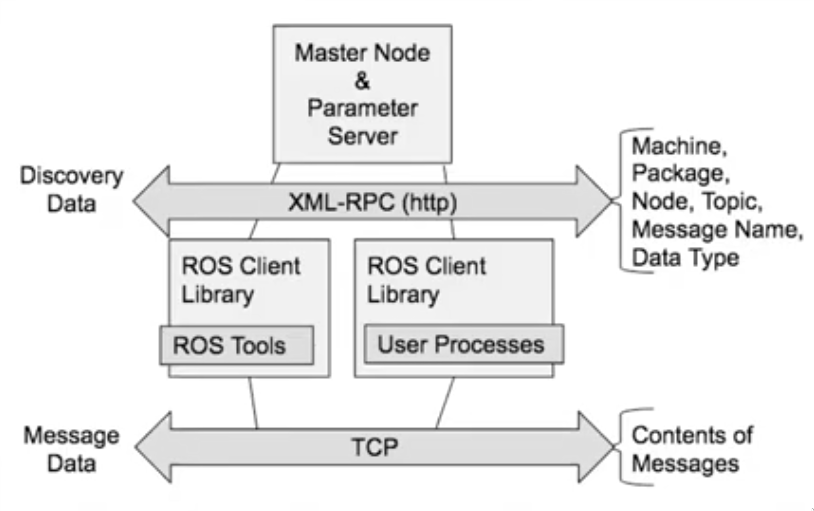
\includegraphics[width=0.6\linewidth]{img/former-ros1-architecture.png}
  \caption{Robot Operating System architecture.}
  \label{fig:ros1-architecture}
\end{figure}

Formerly, due to the sheer wide capabilities controlled by the master, this centralization approach was duly valorized. It naturally fits the purposes of a research tool, as it is simpler to monitor and analyze the system behaviour. However, because it is strongly reliant on the master node's availability, this communication architecture does not scale effectively, making it unsuitable for safety-critical or real-time applications. If the master fails, the entire system fails, representing a single point of failure and a huge performance bottleneck.

Many research communities tried to fix these real-time issues by proposing potential solutions, while supporting the same architecture design. Unfortunately, fell short of meeting the requirements of real-time applications. It became clear to the ROS community that the framework had architectural limitations that could not be rearranged using the same design approach \cite{maruyama2016exploring, dieber2020penetration}.

The \textit{Robot Operating System 2} comes as a complete refactoring of ROS, with the aim of increase the framework's real-time capabilities, by allowing the development of time-critical control over ROS, as it moves away from the former architectural design towards the implementation of an external middleware that can support the production needs of the outgrowing robotic systems \cite{kim2018security, casini2019response}.

\subsection{Data Distribution Service}

The \textit{Data Distributed System} (DDS) \cite{3} is an \textit{Object Management Group} (OMG) middleware standard. The standard was developed to address the demand for enhanced interoperability across different vendors' middleware frameworks, directly addressing data communication between nodes that belong to a \textit{publish-subscribe} communication architecture, for real-time and embedded systems. 

A communication middleware aims to ease the complexity behind creating and maintaining communication architectures. It is responsible for handling relevant aspects like network configuration, communication establishment, data sharing and low-level details. As a result, system developers can mainly focus on their applications purposes, rather than concerning about information moving across levels \cite{dds-what-is}. 

DDS uses the \textit{Data-Centric Publish Subscribe} (DCPS) model as its communication model approach. DCPS is based on a publish-subscribe pattern, where the \textit{data-centric} messaging technique is implemented. It conceptually creates a virtual \textit{Global Data Space}, acessible by any DDS-based application, where data is properly delivered to the applications which quest for it, saving bandwith and processing power \cite{3, pardo2005introduction}. A \textit{domain participant} enables an application to participate in the \textit{Global Data Space}, either as a \textit{publisher} or as a \textit{subscriber}, according to their role on data exchange \cite{maruyama2016exploring, alaerjan2017modeling, dcps-rtps}. 

\begin{figure}[H]
    \centering
    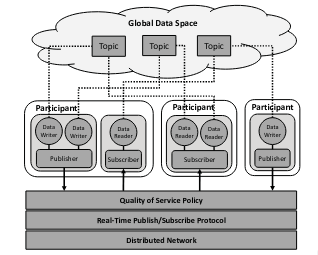
\includegraphics[width=0.4\linewidth]{img/dcps-model.png}
    \caption{DDS architecture: DCPS model with RTPS. Extracted from \cite{maruyama2016exploring}.}
    \label{fig:dcps-model}
\end{figure}

To properly address the data transportation through physical network, DDS offers a wire specification protocol called \textit{Real-Time Publish-Subscribe Wire Protocol} (RTPS) \cite{rtps}, providing automatic discovery between participants. This protocol also works under a publish-subscribe policy over best-effort transports, where data transmission between endpoints is handled \cite{yun2017data}. RTPS allows multiple applications, that could differ on their used DDS implementations, to interoperate with each other as network domain participants \cite{dcps-rtps, alaerjan2017modeling}.

Furthermore, RTPS was designed to employ \textit{Quality of Service} (QoS) profiles, which allow for the specification of various transport policies, formerly not covered by DDS. This approach offers flexibility over communication configuration and development versatility, allowing the developer to specify whatever QoS satisfies its system's communication needs \cite{alaerjan2017modeling, diluoffo2018robot, maruyama2016exploring}. 

Briefly, DDS leverages the premise of a transport-independent virtualized \textit{Data Bus} to address network resources' distribution, in which stateful data is distributed through the network. The involved applications can access this data in motion, representing an architecture with no single point of failure, respectively enabling a realiable way of ensuring data integrity. Consequently, by adopting this approach, the load on the network is independent of the number of applications, making it easily scalable.

\begin{figure}[H]
    \centering
    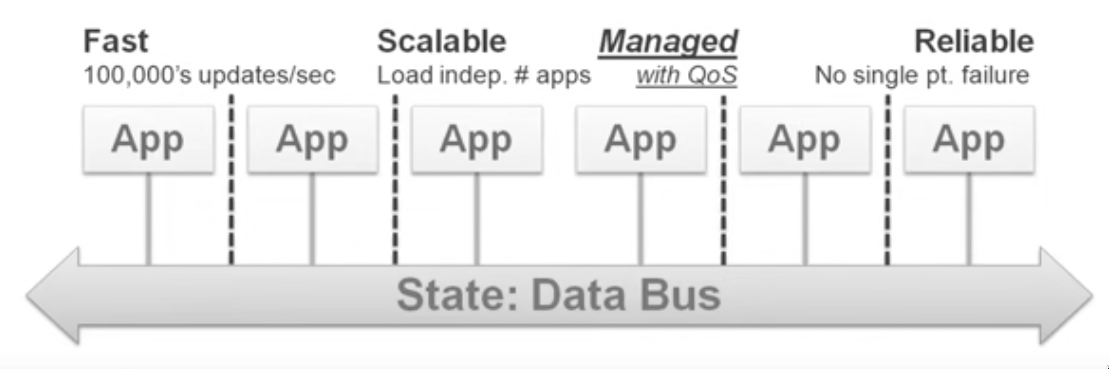
\includegraphics[width=0.6\linewidth]{img/dds-architecture.png}
    \caption{Data Distributed System architecture in a nutshell.}
    \label{fig:dds-architecture-nutshell}
\end{figure}


\subsection{ROS2-DDS Architecture}

As previously stated, the \textit{Robot Operating System 2} was developed to address the former architecture lack of support for real-time systems, mainly due to its architecture design that relied on their own middleware specification. To address this, ROS2 middleware approach is built upon the DDS framework \cite{maruyama2016exploring}, leveraging DDS for its messaging architecture, where communication and transport configuration are handled. 

As far as dependencies are concerned, DDS implementations have light sized dependencies, often related to language implementation libraries, easing the complexity behind installing and running dependencies \cite{ros-on-dds}.

The middleware's on-top layer regards the ROS client library (\textit{rcl}), already implemented in the former ROS architecture. This layer accounts the availability of ROS concepts to the Application layer, as it provides APIs to ease the software implementation by ROS developers \cite{ros2documentation}. As ROS aims to support different programming languages over the same computing context, each language-specficic API must have its corresponding client library (\textit{rclcpp} regarding \textit{C++} and \textit{rclpy} regarding \textit{Python}). The \textit{rcl} accounts these client libraries by abstracting their specification, consequently reducing code duplication \cite{rcl, casini2019response}.

\begin{figure}[H]
    \centering
    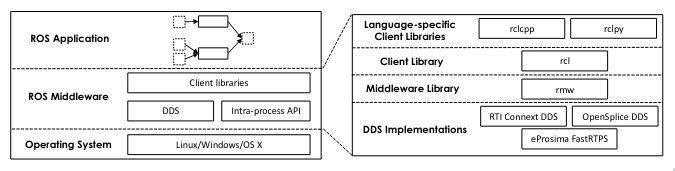
\includegraphics[width=\linewidth]{img/ros2-architecture.png}
    \caption{ROS2 framework architecture.}
    \label{fig:ros2-architecture}
\end{figure}

Towards supplying a wide range of configurations back to application layer, ROS2 aims to support multiple DDS implementations, in which these implementations API specification might differ from each other (currently, \textit{FastRTPS} by \textit{eProsima}, \textit{Connext} by \textit{RTI}, and \textit{Vortex OpenSplice} by \textit{Adlink}). It should be noted that the DDS implementations are low-level of abstraction, strictly defined by its corresponding vendor's API. DDS only defines fundamental procedures at a higher degree of abstraction.  

In order to abstract \textit{rcl} from the specifications complexity of these implementations APIs, an DDS-agnostic interface is being introduced, the \textit{rmw} (ROS MiddleWare) interface \cite{casini2019response}, allowing portability among DDS vendors, which consequently enables ROS developers to interpolate DDS implementations, based on their applications needs during runtime. The information flow through the middleware layer is done over structure mapping between ROS and DDS data models, addressed by the \textit{rmw}, regarding the DDS implementation that is being considered at runtime.

\subsection{Computation Graph}

From a logical perspective \cite{casini2019response}, ROS applications are composed of many software modules that operate as computation nodes, allowing its participation into the ROS \textit{Global Data Space}. The use of publish-subscribe model approach as communication type, through \textit{message-passing} patterns, confers additional concept complexity to the application architecture, where the latter can be naturally represented as a \textit{computation graph} \cite{cousins2010welcome}.

The application's computation graph presents itself as a graphical network, where runtime named entities have their unique role when it comes to data distribution.

\subsubsection{Node Instances}

The application development is done over package orchestrating, where each logically represents a useful software module. Packages might be compromised by numerous \textit{nodes}, that can be perceived as processes that will likely perform computation over the network. It is worth mentioning that, nodes can be connected within a single package or between multiple packages, as they are built over their corresponding packages \cite{cousins2010welcome, intro-ros}.

Thus, the network is comprised by many nodes, running simultaneously and exchanging data between them, where each node addresses its corresponding network module purpose \cite{ros2documentation}. Fault tolerance features are guaranteed as nodes have their corresponding unique name, allowing communication in an unambiguous manner, which confers a suitable approach when developing a complex robotic system.

The notable usage of callback functions provide great functionality when it comes to manage node's behaviour in the communication process. Additionally, \textit{timers} can also be used, since they provide a useful way of managing these callbacks, by time-assigning.

\subsubsection{Communication}

Message-passing is the primary means by which nodes communicate with one another. The \textit{message} definition is a well-typed data structure, which commonly characterizes every data structure concerning the information exchange between nodes. A message is defined by its data type, also known as its \textit{interface}, which can either be primitive (\textit{integer}, \textit{string}, \textit{boolean}, among others), or defined by a complex data structure, where multiple data types are assigned to their corresponding variables \cite{ros2documentation, intro-ros}.

ROS computation graph provides \textit{3} different ways of establish node communication, those being \textit{Topics}, \textit{Actions} and \textit{Services}. These communication mechanisms have different interfaces, specified in different folders with unique namespaces \cite{ros2documentation}.

The concrete mechanisms
\textit{Topics} are perhaps the most common method, naturally perceived as middle-communication buses, over which messages are passed through. As semantic approach, communication through topics is handled by the publishing-subscribing pattern. A node publishes the message to any number of topics, that are then subscribed by nodes that want to get access to that message. Topics provide a multicast routing scheme, where publish data is casted into the multiple nodes that are subscribed to the topic \cite{casini2019response}.

\begin{figure}[H]
    \centering
    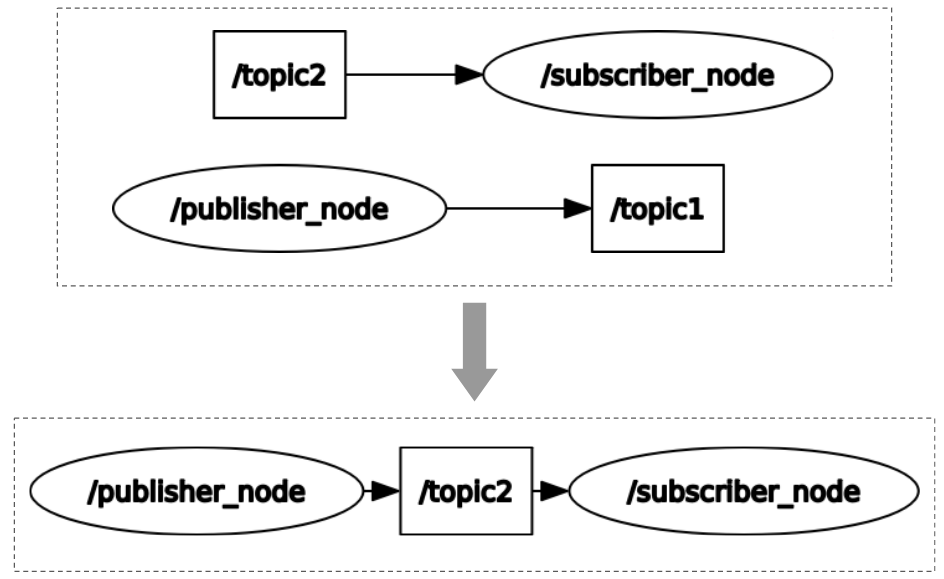
\includegraphics[width=0.5\linewidth]{img/ros2-topics.png}
    \caption{Communication behaviour over \textit{topics}.}
    \label{fig:ros2-topics}
\end{figure}

A specific \textit{topic} is created upon specifying its entity name over either a publisher or a subscriber callback instance. Whenever a node creates a publisher, intentionally instantiated to publish a message through a specified topic, \textit{roscore} is used to advertise the latter, enabling message passing to the corresponding topic subscribers. Message processing is done via the node's callback functions, which are activated upon message receipt, as it can also be utilized for publishing purposes \cite{casini2019response}.

Even though topics are the most conventional way of communication, due to its multicast scheme, subscribers can not be identified by the publishers, so logging and synchronization becomes rather difficult \cite{intro-ros}.

The use of \textit{services} enables a client node, that can also be seen as a topic subscriber, to request data from a server, that likewise a topic publisher, furnish data through a service. This is a bidirectional synchronous form of communication based on a request-response pattern.

Other notable way of exchanging data is by setting goals through \textit{Actions}. Actions are intended to process long-running tasks, where the client sends a goal request to the server node, that confirms the receiving of this goal. The server might provide feedback to the client before providing a response to the client. 


\subsubsection{Launch Files}

A conventional way of deploying a ROS application is through the use of \textit{launch files}, enabling the multi-configuration over entire robotic applications, where network nodes can be individually pre-configurated. Therefore, ROS makes use of the \textit{roslaunch} to automatically initialize the whole network, simultaneously launching each node \cite{intro-ros}. This provides a simpler way of monitoring the system nodes. 

The Figure \ref{fig:ts-rqt-graph} depicts the network architecture corresponding to an ROS application well-known example called the \textit{TurtleSim}. This application is mainly composed by \textit{two nodes}, that perform together towards moving a turtle. Additional nodes were implemented, in order to add complexity to the current network, as to later support security as a proper example. Briefly, the \textit{multiplexer} node acts as a topic selector between two different subscribed topics, where each of them was respectively associated with a priority value. Based on the priority valued, the \textit{multiplexer} node forwards the commands, related to the selected topic, into the \textit{turtlesim} node, triggering the turtle's movement. 

The \textit{rqt} \footnote[1]{ROS provides a GUI tool called \textit{rqt}, that assists developers in manipulating the network elements, in a more user-friendly manner.} visualizer, \textit{rqt\_graph}, allows the developer to perform analysis over a graphical visualization of the network computation graph.

\begin{figure}[H]
    \centering
    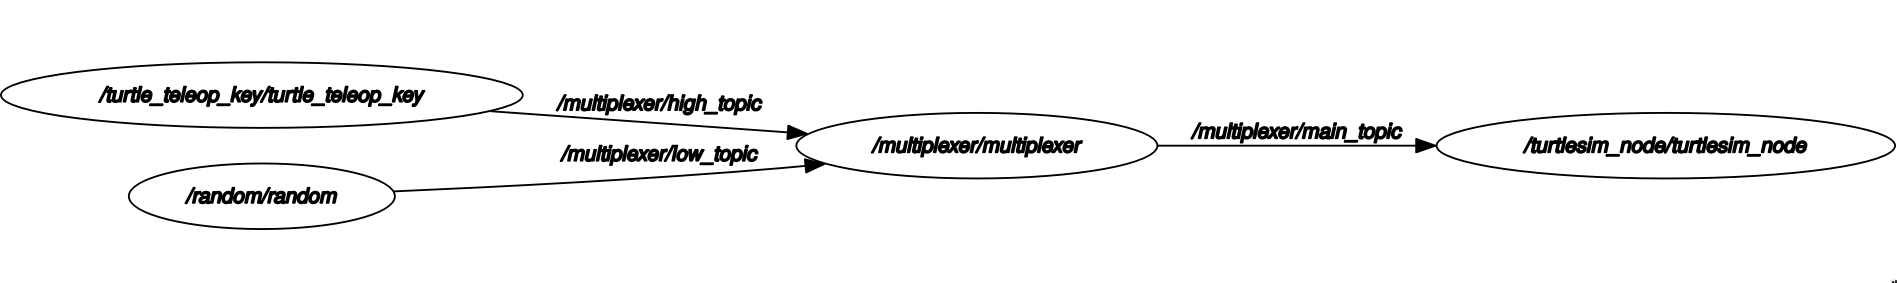
\includegraphics[width=0.8\linewidth]{img/ts_rqt_graph.png}
    \caption{\textit{TurtleSim}'s network graph presented by \textit{rqt\_graph}.}
    \label{fig:ts-rqt-graph}
\end{figure}

After the proper configuration of each node regarding the \textit{TurtleSim} example, the network can be easily managed and automatically launched through a launch file. The Figure \ref{fig:ros-lf} addresses the launch specification related to the latter application.

\begin{figure}[H]
\begin{lstlisting}[otherkeywords={launch, node, name, pkg, exec, output}]
<launch>
    <node name="turtlesim" pkg="default" exec="turtlesim" output="screen"/>
    <node name="keyboard" pkg="default" exec="keyboard"/>
    <node name="random" pkg="random" exec="random"/>
    <node name="multiplexer" pkg="multiplexer" exec="multiplexer"/>
</launch>
\end{lstlisting}
\caption{\textit{TurtleSim} launch file.}
\label{fig:ros-lf}
\end{figure}

Additional node configuration, such as name remapping and parameter adjustments, can be specified under the \textit{args} tag, which offers great functionality to the launching process. 

Distinctive namespaces allow the system to start the nodes, without any name nor topic name conflicts. However, this technique has some flaws attached, since it does not furnish a way of launching nodes in a separated terminal, often needed for user interaction purposes, like input reading.

\subsubsection{Parameters}   

Another relevant concept behind ROS is the existence of nodes \textit{parameters}, that allows individual configuration of the network nodes. In the former version of ROS, the node parameters were controlled by a global \textit{parameter server}, managed by its corresponding ROS Master \cite{intro-ros}. However, in ROS2 each node declares and manages its own parameters, by using the predefined commands \textit{get} and \textit{set}. Additionally, using a parameter function callback, the node's parameters can easily be edited \cite{ros2documentation}.
        
\subsubsection{Node Composition}  

Usually a node is attached to a single process, but it is possible to combine multiple nodes into a single process, structurally abstracting some network parts, while improving the network's performance \cite{ros2documentation}. However, there is a slight difference about how ROS and ROS2 approaches node composition. 

In the former version of ROS, node composition was done over the combination of \textit{nodelets}, intentionally designed to ease the cost of overusing TCP for message-passing between nodes \cite{ros-nodelets}.  Supported by the former idea of \textit{nodelets}, ROS2 introduces the \textit{components} as software code compiled into shared libraries, that can be loaded into a \textit{component container} process at runtime in the network, ensuring node composition \cite{ros2documentation}. 

%Node composition could also be applied for security matters. Suppose a scenario where multiple nodes respect the same security policies. By combining them into a single process, the mapping into this set of rules would be direct, easing the usage of security enclaves.
           

\section{Security}

The deployment of real-time systems implies critical concerning about safety and security \cite{maruyama2016exploring}, resulting of the demanding time-critical scenarios. 

Robotic systems fall under the umbrella of this broad system definition, as they feature unique cyber vulnerabilities related to its integration over highly networked environments, that confers great importance on exposing critical time-reliant scenarios \cite{mcclean2013preliminary, dieber2017security}.

\subsection{Former ROS Security Concerns}

The network security evaluation in a system is done by applying several analyzing techniques. Generally, these techniques do not cover every security aspect, as new vulnerabilities arise from technology evolution \cite{kaeo2004designing}.
The appliance of security countermeasures techniques upon configuring the system's network confers a critical step when aiming towards achieving security.

Within this vast topic, several avenues of endeavor come to mind, each deserving of a substantial study. Network security entails pre-exploration of the system's network through practical networking security techniques, such as intrusion detection and traffic analysis \cite{marin2005network}.

Numerous researchers \cite{8794451, dieber2020penetration} have investigated the use of these techniques, such as port scanning and penetration testing, over the previous version of ROS in order to thoroughly assess attack vulnerability throughout the ROS architecture. 

The ROS Master role in the communication architecture, and its ability to connect to other nodes, imposes many concerns about how to address security to ensure protection over the Master node. Exposing this node poses a critical threat over the whole network \cite{8794451}. 

Moreover, there were also worries regarding the way ROS handled node communication. Network security may be jeopardized, as a result of the publish-subscribe pattern transparency, where node-to-node communications are settled in plain text, making data content vulnerable to unauthorized usage \cite{kim2018security, white2016sros}. Additionally, the former API did not confer any message integrity technique, making applications vulnerable to packet sniffing and man-in-the-middle attacks \cite{white2016sros}.
 
However, due to the high non-linearity and complexity of real-time systems, implementing such thorough analysis method in near real-time remains a significant difficult task \cite{diao2009design}.

\subsection{DDS-Security Specification}

The \textit{Object Management Group} (OMG) \cite{3} accounts security integration by supplying an in-depth specification, consequently adding features to the already developed DDS standard. The \textit{DDS-Security} is a specification that serves as a security extension to the DDS protocol, defined by a set of plugins (Authentication, Access Control, Cryptographic, Logging, Data Tagging), combined in a \textit{Service Plugin Interface (SPI)} architecture \cite{8442103, ros-dds-integration}.

\begin{figure}[H]
    \centering
    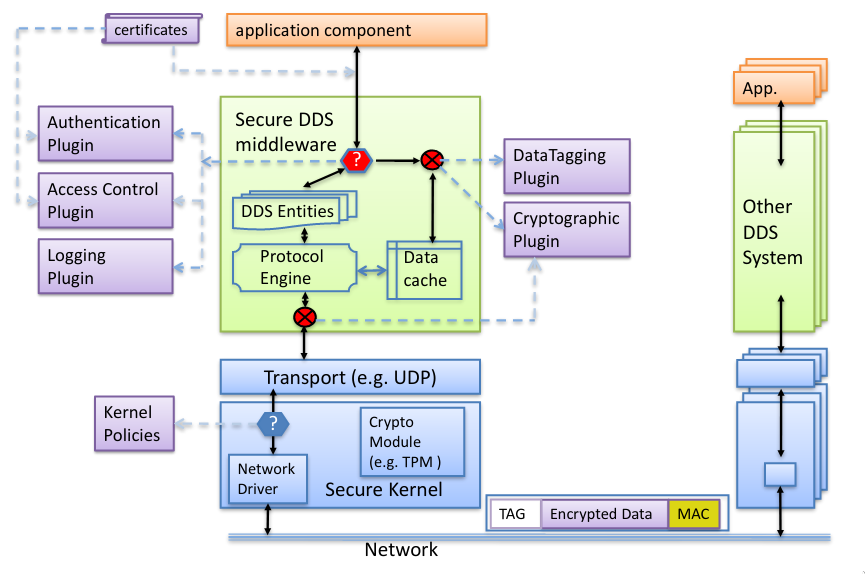
\includegraphics[width=0.7\linewidth]{img/dds-security-architecture.png}
    \caption{DDS-Security Architecture. Extracted from \cite{dds-s}.}
    \label{fig:dds-security-architecture}
\end{figure}

This specification enables its integration by furnishing a \textit{Security Model} supplied to the DDS standard, whereas the \textit{Service Plugin Interface} architecture is responsible for granting plugin enhancement for compliant DDS implementations. Moreover, depending on the security requirements needed for a particular application, these plugins might be adjusted by the latter's runtime DDS implementation \cite{dds-s}.

\subsubsection{Authentication}

Upon considering a secure environment over the DDS \textit{Global Data Space}, data integrity can not be prone to unauthorized usage. Therefore, data exchange requires verification procedures to properly identity the authenticity each DDS domain participant.

The Authentication plugin confers the most valued plugin to the entire SPI architecture, as it provides means to validate the identity of the application, later regarded as a domain participant \cite{dds-s, ros-dds-integration}. 

Each participant must be authenticated prior to entering the data space \cite{white2019network}. Therefore, participants are presented to the secured environment regarding the \textit{Public Key Infrastructure} (PKI). This latter is in charge of issuing asymmetric keys to each participant, a \textit{public} and \textit{private} key respectively, that are used for both authentication and encryption procedures \cite{diluoffo2018robot, ros-dds-integration}. 

Moreover, regarding the issuer identity, the PKI provides an \textit{X.509 certificate}, that maps a distinguished domain name (DN) to the participant's public key \cite{diluoffo2018robot, white2016sros}. This certificate is accountable and signed by a trusted certificate authority (CA) \cite{white2019network, white2016sros, ros-dds-integration}. It ensures authenticity between asymmetric key pairs (both \textit{public} and \textit{private}) \cite{diluoffo2018robot}. 

The communication establishment over different participants must be preceded by a mutual handshake, where keys and certificates are exchanged to guarantee their authenticity \cite{white2019network, kim2018security}. Additionally, the DDS permissions of a domain peer are also concerned within this handshake. The control over permission distribution is respectively handled by the Access Control plugin.

\subsubsection{Access Control}

As aforementioned, the defined DDS specification handles policy control over the DDS domain through the Access Control plugin, where authenticated parties respective operations are imposed by policy restrictions \cite{dds-s, white2019network}. Domains within the \textit{Global Data Space} are controlled over a set of DDS-related capabilities, that are either assigned or restricted to the authenticated participants \cite{ros-dds-integration}. 

Authenticated participants must be granted access to certain domains, where their roles on data transportation must be accordingly accounted by access permissions. If a participant is perceived as a domain data publisher, the domain restrictions must provide publishing privileges to its data topic \cite{white2019network}. 

Following the authentication procedure, domain authorization is also concerned using the proven PKI \cite{ros-dds-integration}, by embedding policy definitions through certificate extensions \cite{white2016sros}. 

Furthermore, the Access Control plugin employs \textit{2} configuration documents that are allocated to each participant \cite{white2019network}. This provides significant security capability, which is given as a supplement to the authentication procedure.

\textbullet\ Domain Governance: \textit{XML} document defining the domain's security policy.

\textbullet\ Participant Permissions: \textit{XML} document containing the permissions assigned to a given domain participant.

Notably, these configuration files are signed by a trusting Certificate Authority (CA) \cite{ros-dds-integration}. The CA's Permission Certificate confers protection against elevation of privilege attacks. Therefore, if the policy integrity is jeopardized, the handshake establishment between authenticated parties fails to commence \cite{white2016sros}.

\subsubsection{Communication and Encryption}

% The DDS-Security specification ensures encryption and authentication using \textit{OpenSSL}, while accounting security functions based on encryption standards \cite{takemoto2019performance}. Accordingly, it implements a handshake-based standard, concerning the \textit{OpenSSL} protocols, \textit{Secure Sockets Layer} (SSL) and \textit{Transport Layer Security} (TLS), which are used respectively used to ensure encryption over the network communication \cite{white2016sros, kim2018security}.

%The handshake is used to achieve mutual authentication within participants over the DDS domain. As stated, each participant must be authenticated prior to entering the data space \cite{white2019network}. Therefore, participants are presented to the secured environment regarding the Public Key Infrastructure (PKI). This latter is in charge of issuing a public certificate, accountable and signed by a trusted certificate authority (CA) \cite{white2019network, white2016sros}.

The DDS-Security specification ensures encryption and authentication using \textit{OpenSSL}, while accounting security functions based on encryption standards \cite{takemoto2019performance}. 

Accordingly, it implements a handshake-based standard, concerning the \textit{OpenSSL} protocols, \textit{Secure Sockets Layer} (SSL) and \textit{Transport Layer Security} (TLS), which are used respectively used to ensure encryption over the network communication \cite{white2016sros, kim2018security}. The handshake is used to achieve mutual authentication within participants over the DDS domain \cite{white2019network}.

Following the participant key assignment, the \textit{Diffie-Hellman} key exchange protocol properly accounts the mentioned handshake, allowing both participants to exchange data over a shared secret key \cite{kim2018security}. % while accounting their own public certificate information \cite{kim2018security}. 
It enjoys the inter-exchange of both asymmetric keys, issued to each domain participant during the domain authentication procedure, in order to perform sign (using the private key) and verify (using the public key) operations \cite{kim2018security, diluoffo2018robot}.

The \textit{rcl} is capable of handling this DDS security requirement, levering ROS-based applications to support SROS2, accounting nodes as authenticated participants \cite{white2016sros}. 

As communication establishment is duly achieved throughout this handshake process, the DDS-Security specification takes advantage of the \textit{AES-GCM} encryption standard concerning data encryption over the implicit channel \cite{kim2018security, takemoto2019performance}.

\begin{figure}[H]
    \centering
    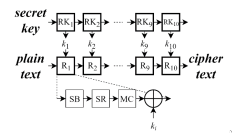
\includegraphics[width=0.4\linewidth]{img/ros_aes.png}
    \caption{\textit{Advanced Encryption Standard} algorithm. Extracted from \cite{takemoto2019performance}.}
    \label{fig:ros_aes}
\end{figure}

The \textit{key cryptosystem} algorithm \cite{takemoto2019performance} presented in the \textit{Advanced Encryption Standard (AES)} considers the usage of functions towards achieving data encryption over the established communication. It enables configuration over data encryption, allowing both block and streaming transfer of ciphered data \cite{diluoffo2018robot}.

Here, the algorithm combines the shared key established with the message passed over the secure channel. Moreover, it is desirable to implement the \textit{Galois MAC (AES-GMAC)} encryption algorithm, that is based on block cipher operations, consequently adding encryption functionality to the AES algorithm, through a \textit{Message Authentication Code (MAC)} encryption function \cite{takemoto2019performance, kim2018security}.

Every cryptography-related operations are handled by the SPI's Cryptographic plugin. Naturally, these cryptographic capabilities, linked to the asymmetric key cryptography, are then used by both Authentication and Access Control plugins, ensuring authenticity support over their corresponding opeartions \cite{ros-dds-integration, diluoffo2018robot}.

\subsection{Security Integration in ROS2}

As result of the \textit{Data Distribution Service} (DDS) implementation as a flexible middleware interface in the ROS2 architecture, issues regarding security is no longer mainly ROS-dependent. Thus, when it comes to addressing security over communication, and subsequently data protection enhancement, ROS2 is heavily reliant on how the DDS standard is able to manage security \cite{kim2018security, 8794451}.

Every DDS implementation supported by ROS2 makes use of the DDS-Security specification, enabling security over ROS's application environment. Even though ROS2 is deployed without security mechanisms by default \cite{ros-dds-integration}, ROS2 provides a toolset, the \textit{Secure Robot Operating System 2} (SROS2) toolset \cite{sros2-gh}, extending ROS2's functionality to make use of the DDS-Security functionality. 

The control over these tools are done by \textit{rcl}, providing security over the Application layer, while DDS is capable of providing security over the communication architecture \cite{kim2018security}. SROS2 configuration is done over applying a set of security files to each ROS2 participant, with regard to how DDS handles certificate assignment to their participants \cite{white2016sros, ros-dds-integration}. 

Consequently, the toolset allows certificate generation and allocation through a keyserver directory, where security enclaves and their respective authentication files are stored inside subfolders \cite{white2016sros, ros-dds-integration}. Moreover, SROS2 enables the keyserver configuration in a flexible way, allowing developers to restricit certificate and CA attributes to an arbitrary number of nodes, defined over the same namespace \cite{white2016sros}.

The variety of capabilities in SROS2 toolset attempts to aid with security configuration across environments \cite{ros-dds-integration}. However, managing certificates and access control policies might lead to improper configuration. Additionally, orchestrating a real-time network towards achieving a secure environment confers to be a demanding process \cite{ros-dds-integration, white2019network}.

% The SROS2 configuration is done over applying a set of security files to each ROS2 participant, with regard to how DDS handles certificate assignment to their participants \cite{white2016sros}. The variety of capabilities in SROS2 toolset attempts to aid with security configuration across environments, however, the developer must be aware of improper configuration, that can still lead to security problems \cite{ros-dds-integration}.

\subsubsection{Security Enclaves}

As aforementioned, ROS2 relies on how handles DDS security over their \textit{Domain Participants}. DDS imposes the authentication of each participant prior to joining its \textit{Global Data Space}, where the Certificate Authority and an established PKI comes in hand \cite{white2019network, white2016sros}.

Accordingly, the authentication process within the ROS2 network relies on the notion of a network enclave, where authentication and control artifacts are stored to properly achieve security over the network data space \cite{ros-security-enclaves}. Conceptually, an enclave is a secure region in the application address space that maintains confidentiality and integrity, while computations are being carried out on data.

Previously, a node was perceived as a separated DDS participant. However, by considering node composition as a reliable way of matching multiple nodes simultaneously to the same security domain, this node perception as participants can not be taken into account, due to causing non-negligible overhead, as memory space becomes rather difficult to handle \cite{ros-security-enclaves, ros-access-control}.

Concerning the enclave authentication procedure, its security artifacts must be addressable by a DDS participant, where the latter is associated to a node sharing context, instead of being perceived as a single node \cite{ros-security-enclaves}. Thus, when it comes to apply different policies over different nodes, that are matched in the same node context, a set of node \textit{profiles} can be specified under the enclave notation. 
 
\vspace{0.5cm}
\textbf{Access Control within Enclaves}

The SROS2 toolset offers a well-typed markup language \textit{XML schema} \cite{ros-access-control}, where security policies bind profiles to access permissions for network objects, granting privileges back to a certain profile. \textit{Profiles} are implemented under the \textit{enclave} declaration, to duly support the node composition into a single process, enabling the possibility of combining multiple profiles, respectively addressing its corresponding node. % Typically, each \textit{enclave} declaration is linked to a corresponding ROS node, naturally perceived as a DDS participant.

\textit{Objects} are classified over a subsystem type, structurally characterized by permissions tags. Then \textit{object privileges} are controlled over access values, either \textit{allow} or \textit{deny}, attributed to their corresponding permissions tags \cite{ros-access-control, white2018procedurally}. Briefly, each node profile is assigned to policies that concern some object identifier (OID). Each OID maps to a specific action, that is identified over an access value, allow or deny respectively \cite{white2016sros}.

The policy design approach works under the \textit{Mandatory Access Control} (MAC), that denies any privilege by default. The only way of allowing access to any object, is by explicitly specifying the subject's privilege access \cite{ros-access-control, white2018procedurally, white2016sros}. Naturally, this policy approach confers great value towards security, since it denies any attempt of privilege gaining attack by ROS-based packages from non-trusted sources \cite{white2016sros}.

Depicted in the Figure \ref{fig:ros-access-file}, it is presented a policy file where access control privileges are distributed across enclaves, and their inherited profiles. Recall the \textit{TurtleSim} example, the following \textit{XML} policy file addresses the access to topics for each respective enclave. 

\begin{figure}[H]
\begin{lstlisting}[otherkeywords = {xml, version, encoding, policy, version, enclave, enclaves, profile, profiles, topic, topics, xmlns:xi, path, ns, node, publish, subscribe, reply, request, call, execute, xi:include, href, xpointer}]
<?xml version="1.0" encoding="UTF-8"?>
<policy version="0.2.0" xmlns:xi="http://www.w3.org/2001/XInclude">
  <enclaves>
    <enclave path="/multiplexer">
      <profiles>
        <profile ns="/" node="multiplexer">
          <topics publish="ALLOW" >
            <topic>move_turtle</topic>
          </topics>
          <topics subscribe="ALLOW" >
            <topic>high_priority</topic>
            <topic>low_priority</topic>
          </topics>
        </profile>
      </profiles>
    </enclave>
    <enclave path="/turtlesim">
      <profiles>
        <profile ns="/" node="turtlesim">
          <topics subscribe="ALLOW" >
            <topic>move_turtle</topic>
          </topics>
        </profile>
      </profiles>
    </enclave>
    <enclave path="/keyboard">
      <profiles>
        <profile ns="/" node="keyboard">
          <topics publish="ALLOW" >
            <topic>high_priority</topic>
          </topics>
        </profile>
      </profiles>
    </enclave>
    <enclave path="/random">
      <profiles>
        <profile ns="/" node="random">
          <topics publish="ALLOW" >
            <topic>low_priority</topic>
          </topics>
        </profile>
      </profiles>
    </enclave>
  </enclaves>
</policy>
\end{lstlisting}
\caption{SROS2 policy file regarding the access control policies over the \textit{TurtleSim} example.}
\label{fig:ros-access-file}
\end{figure}

\section{Related Work}\label{s:relWork-sec}

The present section confers a notable overview over ROS security environment, that will focus on the following topics: It is intended to begin by presenting some works that demonstrate the absence of security over the ROS environment, that is then followed by some attempts regarding solutions; At last, ROS2-based studies will be given to contextualize the dissertation's main topic of study. 

Robotic systems were initially conceived as augmented computers with no explicit boundaries or limitations. As a result of the requirement to provide practical systems as fast as possible, security matters were disregard \cite{white2018procedurally}. Network security entails cautious analysis of the system's network using realistic networking security procedures \cite{marin2005network}. Concerning the Robot Operating System and its role as a robotic application enhancer, numerous researchers have examined the usage of such procedures to perform a thorough analysis over the latter's architecture.

\citeauthor*{8794451} presents a practical overview over ROS security, in which the \textit{IPv4 address space of the Internet} is explored with the goal of identifying vulnerable hosts. Port scanning was used as technique to expose mostly master nodes as they provide valuable information about their associated topics and node's parameters. The performed scans furnished information about hosts that could either be a sensor, an actuator or even a simulator. This study is rather relevant because of how easily can attackers gather information about potential robots, and control them further on, through the public Internet, making it unavoidable to develop mechanisms concerning security. 

Moreover, in \citenum{dieber2020penetration}, it is presented different pentesting tools that entails exploiting techniques over ROS-based systems, in order to provide a proper overview of possible security flaws. Foremost, \citeauthor{dieber2020penetration} presents a \textit{.net-based pentesting} tool called \textit{ROSPenTo}, developed with the intention of investigating strategies for manipulating running ROS applications. The latter provides several command line techniques to jeopardize robotic networks, including the ROS parameter server, that confers great value to the running nodes. 

The other tool is called \textit{ROSchaos} wittingly designed for exploiting the Master API. It differs from the former tool, since \textit{ROSPenTo} mainly focused on exploiting ROS \textit{Slave API}, which covers the node-to-node communication and the receipt of messages from the Master, without directly addressing the ROS Master as a compelling target. Regardless matter how subtle such attacks are, exploiting the Master directly may still be appealing to attackers. 

These techniques confer great value to the domain of security exploration over ROS, where the \textit{XML-RPC} embedded API is divided and subsequently exploited according to the participants roles within the network. Besides raising awareness of the importance of security in ROS, it promotes developers to conduct penetration testing on their applications.

Following the challenges that arose as a result of executing exploitation techniques on the ROS framework, numerous solutions were proposed in response to the need to offer security assurance for robotic applications. 

One of the earliest research on the security improvement of the ROS framework was proposed by \citeauthor{mcclean2013preliminary} in \citenum{mcclean2013preliminary}. Here, the first take is to exploit and reason about unique vulnerabilities related to the nature of cyber-physical systems, where it is demanding to collect data for further consideration. Afterwards, it is presented a novel research tool to aid in cyber-physical security research, named as \textit{honeypot}, where it is desirable to monitor unauthorized attempts to jeopardize these systems. Due to the significant information offered, the latter gives a basic yet crucial study on ROS, which acts as assistance to steer the development of future work in the burgeoning subject of cyber-physical security. 

% Another worth-mentioned research is presented in \citenum{crick2017rosbridge}. The latter describes the \textit{rosbridge} middleware that adds to the former ROS architecture an abstraction layer. It provides a socket-based interface through a technology standard, where minimalist services are accessible to developers.

In \citenum{white2016sros}, \citeauthor{white2016sros} addresses the security deployment over ROS in a more concise way, by proposing the \textit{Secure Robot Operating System} (SROS) as a planned enhancement to the former API, that includes mechanisms such as authentication, access control and cryptography measures. SROS seeks to provide adequate security architecture while minimizing existing user disturbances such as computational cost and API breaking. The final remarks regard the alternative usage of SROS, allowing developers to customize it to their own internal certificate formats. Moreover, \citeauthor{white2016sros} expects security logging and access control to evolve through well-defined standards, enabling more robust auditing and policy generating tools. 

Additionally, in \citenum{application-security-ros} it is presented a fairly pertinent research that recommends security improvements on the application-layer. Briefly speaking, the approach primarily focused on applying security measures on the application layer, by mainly running an Authentication Server, storing certificates and files related to trusted domain participants, while controlling and providing session keys related to the communication process. Topic-specific encryption keys are employed to protect data secrecy. However, the discussed architecture is based on the assumption that issuing authentication certificates are manually handled. Despite encryption and authentication mechanisms, attacks regarding the exposure of the network, such as denial of service attacks, still persist which cannot be handled on the application level alone. 

\citeauthor*{breiling2017secure} continues to follow the previous work in \citenum{breiling2017secure}, through a hardened ROS core with transparent authentication, authorization, and encryption functionalities that do not require the manual specification of nodes. Furthermore, secure workflows and initial penetration testing are supported in \citenum{dieber2017security}, in which \citeauthor{dieber2017security} shows an insight of security weaknesses in the ROS architecture design, with additional attempts that regard potential solutions to those problems.

Regarding the SROS \cite{white2016sros} initial proposal, \citeauthor{white2018procedurally} continued to provide security overview over the framework through subsequent studies \cite{white2018procedurally, white2019network}. In \citenum{caiazza2019enhancing}, \citeauthor*{caiazza2019enhancing} presents several solutions regarding the lack of security measures that autonomous devices, often related to the robotics world, tend to face. The effort then moves on to evaluate the ROS framework in order to provide a high-quality understanding solution. It follows a pipeline of security measurements, where logging, access control and authentication certificates are discussed over several proposals. It provides a clear analysis over the security state-of-art of ROS, and the analysis clearly states that the lack of techniques to prevent communication threats imposes the most valued consideration over robotic networks. \citeauthor*{caiazza2019enhancing} conclude their work by stating some future improvements to their current solution. 

In \citenum{white2018procedurally}, \citeauthor*{white2018procedurally} addresses robotics security through a proposed framework that focuses on handling access control policies for robotic software, with the intention of adding functionality to SROS \cite{white2016sros}. The latter offers an interesting perspective on leveraging access-control through a well-typed markup language schema, the \textit{ComArmor} configuration language, where privileges of objects is explicitly defined over policies. Then, profiles are used to arrange these policies in a hierarchical manner, binding namespaces to objects privileges, utilizing attachment expressions with predefined permissions denoted as rules. Rules are defined as a set of permissions for a given object, where each permission has a corresponding value that could either be allow or deny. 

The evaluation of this policy schema as a proof of concept was done by implementing it in a cryptographic framework called \textit{Keymint}. The latter follows similar authentication and cryptographic patterns as the initial SROS \cite{white2016sros}, where security artifacts and document keys are stored in respective keystores. The incorporation of the ComArmor language into Keymint adds significant value to the framework since it allows for reasoning about how to manage policy control prior to implementing any authentication mechanism, such as generating permission and governance files. The framework is then tested using a standard ROS example of a basic publisher and simple subscriber interacting over a topic. Thus, this approach provides a methodical testing procedure where both application satisfiability and access control policies implementation are overviewed, adding significant value back to the framework as it is possible to define higher level policies to allow for transport-independent access control definitions.

The \textit{ComArmor} configuration language, presented above in \citenum{white2018procedurally}, confers a great alternative to the SROS2 default policy schema. During the framework's evaluation process, \citeauthor{white2018procedurally} presents a set of gratuitous permissions within SROS2 template through a simple comparative study between both configuration languages. Thus, it discusses possible SROS2 vulnerabilities discovered during the development and experimentation the \textit{Keymint} framework, emphasizing the importance of continuous security evaluation throughout design development cycle.

Following the deployment of DDS in Robot Operating System 2, the majority of security problems were alleviated. As a result, the literature on the network security enhancements provided by ROS2 is largely concerned with providing an overview of the trade-off between performance and security. Furthermore, various inquiry studies evaluate ROS2 performance in terms of response time and safety important circumstances \cite{maruyama2016exploring, casini2019response}, in which DDS capabilities are highly emphasized to properly evaluate ROS2.

A notable work is presented in \citenum{kim2018security}, where the security definition of DDS was explored using current security standards. Also, the implementation of the DDS protocol was evaluated using techniques of static analysis. It provides a framework for doing benchmark evaluations in various network and security configurations to reflect on the needs of real-time applications. Different performance time-related metrics and benchmark network scenarios (wired and wireless) were thoroughly investigated to give a well-based analysis over efficiency. The findings clearly illustrate that employing a reliable VPN application is more time efficient; nevertheless, SROS offers far more decentralized features than a VPN, which is typically desirable when designing a distributed system. \citeauthor*{kim2018security} conclude their work by reasoning about the security capabilities that DDS has to offer, after which a static code analysis of the DDS security implementation was undertaken. The research revealed that the latter did not conform to the security specfication by OMG. 

A pertinent research that examines the trade-off between performance and security is regarded in \textit{Robot Operating System 2: The need for a holistic security approach to robotic architectures} \cite{diluoffo2018robot}. Here, \citeauthor{diluoffo2018robot} conducts a thorough examination of Robot Operating System 2 and outlines possible hazards for this new robotic system paradigm. Thus, the DDS security specification is thoroughly examined in terms of performance versus security models and how security is integrated with ROS 2, as well as how the addition of security affects system design. 

As a result, \citeauthor{diluoffo2018robot} goes on to present a systematic study of ROS2 in order to provide a good knowledge of how the system is built, and to subsequently undertake vulnerability analysis across various layers that require varying levels of protection. Additionally, the authors applied different performance metrics to duly present a well-based comparasion in whether security should be considered or not. Here, they consider the usage of DDS-based implementations, while addressing the RTPS communication protocol and it handles the communication and its configuration. The experiment illustrates that implementing security measures on protected data in motion results in a significant performance loss. 

Notably, they conclude with some recommendations towards security areas not duly covered by the DDS specfication, such as attacks stemming from
spy processes. They highlighted the preservation of the cognitive layer because of its importance in the robot itself, since all types of sensors that involve data collecting are concerned in that layer. Here, an advanced set of threats were described using Machine Learning, in which DDS is not capable of cover.

These presented works denote important considerations about how important is to address security over robotics, due to the variaty of attacks that might compromise their integrity. They follow the path of addressing vulnerabilities through applying security methods based on tools and protocols. However, studies regarding the appliance of quality analysis over static and property verification in ROS are quite limited. Despite this, the section \ref{s:relWork-pv} contains several works that advocate utilizing quality analysis to assess robotic systems.

\chapter{Alloy Specification Framework}\label{c:alloy}

As aforementioned, this dissertation aims to tackle the security vulnerabilities resulted from the miss-configuration over ROS files. In this chapter, it is intended to explore the Alloy framework that is relevant to overcome the above-mentioned challenge. % as well as previous developed work that has the same or similar goals as this thesis (\ref{s:alloy-relWork}).

The increasing usage of robotics onto safety-critical systems results in demanding considerations over ensuring the proper correctness of both software and hardware, as failures often leads to fatal consequences, especially regarding the security domain. Thus, the use of formal methods and verification techniques, especially in systems highly reliant on flexibility and reliability, is recommended to avoid security-critical faults \cite{clarke2011model}. Software frameworks designed for this purpose must provide methods to perform structural design over systems with rich structures, abstracting their behaviour as a conventional model. Additionally, these frameworks must support features to enable automate analysis, in which property evaluation over these designed models is used as technique. 

The \textit{Alloy Framework} \cite{alloy-DJ}, fits within this context, as it furnishes a declarative relation-based language, used for software modelling, complemented with extended tools supporting analysis over these models \cite{alloy-6}. The language combination of both \textit{Relational} and \textit{Linear Temporal Logic} (LTL) enables the ability to model both systems with rich structures and complex behaviour. To address the correctness over the specified model, Alloy performs model-checking techniques over these logic languages, where the model $M$ is exhaustively checked over property verification \cite{lwspecification}.

The framework \textit{analyzer} takes the specified model's restrictions into account, performing \textit{Bounded} and \textit{Unbounded} Model Checking to find instances that satisfy those implied restrictions. It can be also be useful for checking model properties, where the analyzer will try to return a counterexample instance. Instances are displayed by the framework Visualizer, alongside with the modelling process steps, regarding a trace representation. Instances appearance can be customized, using the \textit{theme}'s extension \cite{alloy-6}.

This chapter will go through these principles in further depth, to give the reader a proper review on how Alloy is structured, as its importance as a model checker to the computation domain, supported by a previously configured example where ROS communication architecture is structurally modelled. Since system analysis rely on the reasonable implementation of Model-Checking techniques, the following section within this subject intends to cover a clear contextualization on this matter. % since it is highly important on understanding how Alloy's verification process works.

\section{Model Checking}

% Model-checking is increasingly popular in the early phases of the software development process. To establish the cor- rectness of a software design one must usually verify both structural and behavioral (or temporal) properties. Unfor- tunately, most specification languages, and accompanying model-checkers, excel only in analyzing either one or the other kind. This limits their ability to verify dynamic systems with rich configurations: systems whose state space is character- ized by rich structural properties, but whose evolution is also expected to satisfy certain temporal properties. To address this problem, we first propose Electrum, an extension of the Alloy specification language with temporal logic operators, where both rich configurations and expressive temporal properties can easily be defined. Two alternative model-checking techniques are then proposed, one bounded and the other unbounded, to verify systems expressed in this language, namely to verify that every desirable temporal property holds for every possible configuration.

Performing software testing has been regarded as the established assessment procedure in which functional and non-functional specifications are evaluated. The conventional approach on software verification is based on testing the system with different inputs, to achieve quality assurance over several intended specifications \cite{beyer2017software, briand2001uml}. As this technique demands exhaustively evaluation over pre-selected test data, it is commonly explored over automated tools, since manual testing is time-consuming and prone to errors \cite{clarke1976program, fraser2009testing}.

% Model-based testing arises as a viable alternative technique, in which both test cases and intended behaviour relies on the design of an abstract mode, presenting remarkable benefits to the latter approach. \cite{apfelbaum1997model} Thus, to perform full verification over systems, the \textit{model-checking} technique can be used to automatically interpret counterexamples as test cases, consequently enabling far better degrees of coverage than conventional testing. \cite{fraser2009testing, beyer2017software}

\textit{Model Checking} presents itself as a novel technique with the purpose of verifying temporal properties over the system finite-state, with the latter being duly represented as a conclusive model. Additionally, it enables \textit{model-based testing} by automatically interpreting counterexamples as test cases, resulting in significantly greater degrees of coverage than conventional testing \cite{fraser2009testing, beyer2017software}. This technique is becoming highly used due to its importance as an early phase approach upon developing systems \cite{lwspecification}, as it confers the most valued functionality over model-checking frameworks, in which concrete models, regarding the software architecture, is exhaustively checked over behavioural properties. 

It provides highly automatic verification procedures, where other techniques, such as theorem provers fails to address, due to its deductive reasoning nature. The representation of not satisfied specifications over counterexamples, confers great functionality to this technique, often required for debugging matters.
However, the system's inevitable state expansion consequently causes the complexity increase on verification. This is referred to as the \textit{state explosion problem}, in which model-checking is unable to handle the size of the state space \cite{clarke2011model, clarke1997model}. Yet, this is can be mitigated using bounded techniques.

Model Checking techniques accounts property verification of systems through the implicit use of temporal logic to express \textit{dynamic} behaviour through the course of the system evolution. Thus, the system must be abstractly represented as a transition system, perceived as concrete models, to perform property checking over the latter, while considering the formula defined in a temporal logic \cite{huth2004logic, vakili2012temporal}. 

\vspace{0.5cm}
\textbf{Transition System}

A \textit{Transition System} is defined over a graph-based structure, that confers additional representation over the mathematical graph structure. The latter offers weak ability to provide a concrete system description over a discrete model. Commonly, transition system confers a labelling function that maps each state, naturally perceived as graph node, with so-called \textit{atomic propositions}. These propositions evaluate system variables in each state \cite{muller1999model, vakili2012temporal}.

\textit{Kripke Structures} were intentionally conceived to address the model checking field of action, so they naturally fall under the umbrella of this vast domain \cite{muller1999model}.

Conceptually, a \textit{Kripke Structure} defines a model $M$ with the following tuple structure $M = (S,I,R,p,L)$, where: $S$ is a finite set of states; $I$ represents a set of initial states, so naturally $I$ is a subset of $S$ ($I \subseteq S$); $r$ defines the \textit{transition relation} as it accounts the transitions between states; $L$ is an \textit{interpretation} that defines the labelling function; Accordingly, it assigns each state with a set of valid atomic propositions $p_{s}$ enjoyed by it, draw from the domain of $p$ ($p_{s} \subseteq p$). 

\vspace{0.5cm}

Model Checking is a \textit{model-based} technique in which property verification concerns are centered on the concept of \textit{satisfaction}. Therefore, the corresponding model-checker must be capable of checking if the model $M$ satisfies a desirable property, expressed as temporal logic formula $\psi$. As this computing process relies on a state representation, the formula verification also accounts a model state $s$. $M,s \models \psi$ \cite{huth2004logic, muller1999model}.

Additionally, the semantics of the temporal logic relies on how the latter addresses time as an evolving approach towards state verification. Notably, temporal logics are either qualified as \textit{linear-time} or as \textit{branching-time} \cite{huth2004logic}. In the former approach, time is perceived as linear path and the corresponding transition system is abstracted by a set of infinite traces. The latter denotes time as a branching model, in which the transition system is abstracted by a set of infinite computation trees, consequently enabling non-deterministic considerations about the system evolution. The choice on the logic semantics relies on the system properties to be analyzed \cite{muller1999model}, as they confer different model-checking algorithms \cite{huth2004logic}. 


% \subsection{Model Checking in Alloy}
% 
% Following the temporal logic semantics, Alloy specification language embeds the linear temporal logic into the first-order logic, thus, it makes use of both temporal and relational quantifiers to properly express behavioural verification over time \cite{lwspecification}. \textit{First-Order Temporal Logics} present additional techniques for reasoning about behaviour, while accounting the basis of the first-order logic, that usually confers the capability to express the well-formedness of the system structure \cite{lwspecification, konur2010survey}.
% 
% The \textit{FOLTL} syntax confers bounded and unbounded semantics, in which 
% 
% The Alloy Framework performs model checking through \textit{2} distinct techniques, those being the \textit{Bounded} and \textit{Unbounded}, already introduced earlier in this section, to verify that temporal properties hold considering the model specification \cite{lwspecification}. 
% 
% Usually, the \textit{Bounded} model checking is considered as first approach to validate the model specification. In addition, performing \textit{Unbounded} model checking proves to be a novel approach to check the model consistency, as it provides high degrees of reliability due to its verification coverage. 

\section{Structural Design}

The \textit{Alloy framework} presents itself as a formal modelling language, conceived to properly address model-checking techniques over their specification language, where both structural design and temporal behaviour, naturally specified over properties, can easily be defined. Formerly, Alloy was inherently static \cite{lwspecification}, meaning that it only excel the structural design, where its language was based on first-order logic. The analysis process relied on a bounded model checking technique with no support for temporal behaviour. Notwithstanding, the latest release of Alloy confers the ability to properly deal with expressive temporal properties, as well as trace evaluation over time, while employing the former structural approach. 

As intentionally design to formally abstract both system's configuration and behaviour, Alloy successfully incorporates a set of features, within a well-documented and wide-ranged syntax that consequently allows large specification development \cite{lwspecification}. The following subsection \ref{c:alloy-sm} addresses the Alloy concepts required for understanding how system modelling is covered. 

\subsection{Structural Modelling}\label{c:alloy-sm}

Alloy aims to address the complexity behind richly structured systems, that require critical control over their intended behaviour, by presenting a novel approach for abstracting these systems as conventional models. 

System's structures can be specified over time-evolving states, where its behaviour clearly identifies the states' inbetween transitions. The conception of system transitioning offers a great formal approach when it comes to reason about the system's design.

The Alloy structural definition relies on a relation way of connecting system's elements, where the latter is abstracted in terms of relations. In Alloy, unary relations, commonly known as sets, are labelled as \textit{signatures}, that are inhabited by a set of \textit{atoms}, from a finite universe of discourse. Atoms are perceived as the lowest-grain elements, with no particular semantics attached. A signature, identified by the keyword $sig$, might include multiple \textit{field} declarations enclosed between braces, addressing relation between the signature's atoms and a set or other relation. Fields are inhabited by tuples of atoms from the universe, that must meet the same arity.

Signatures can either be perceived as a top-level signature, or as other signature's subset. Signature hierarchy is conceivable through disjoint extensions ($extends$), or by set inclusion ($in$). The $abstract$ keyword declares a signature that contains no atoms beyond those within its extensions. 

To address default configuration over the universe's multiplicity, both signatures and fields can be specified under a multiplicity constraint. The former constrains the number of signature atoms, where it is commonly used to express singleton sets, over the constraint keyword $one\ sig$. Fields, however, makes great use of multiplicities by restricting behaviour over relations between atoms. In addition to these model constraints, explicitly specified over the course of the modelling process, system assumptions can be defined over axioms, expressed as $facts$, where multiple constraints can be incorporated \cite{gheyi2007formally}.

Moreover, the latest Alloy version enables evaluation changing throughout the trace evolution, consequently allowing the consideration of both signatures and fields as time mutable declarations, through the usage of the keyword $var$.

Throughout the sections that follow, it will be presented an illustrative example over which graph theory rests, this being the study of \textit{Eulerian Circuits}. This example will be used to duly contextualize both modelling and verification process in Alloy. \textit{Eulerian Circuits} must meet several behaviour constraints over the classic graph definition, that must be addressed over model constraints. However, the structural modelling must be provided beforehand.

\subsubsection{Model Structure}

With regard to the presented example, as it falls under the study of graphs theory \cite{west2001introduction}, it follows an abstract representation of the graph mathematical structure. In this sense, a graph is made up of nodes which are connected by edges. 

Considering the Alloy's abstract ability to reduce complexity over model designing, at a high degree of abstraction, graphs can be represented as a set of \textit{nodes}, that connect together over relations, with no need to address edges as a separated structure declaration. 

\begin{lstlisting}[title={Graph representation over a sigle Node declaration.}, otherkeywords = {abstract, sig, module, var, set, fact, extends, no, in}, label={lst:node},floatplacement=H]
sig Node {
    adj : set Node, 
    var visited : set Node
}
\end{lstlisting}

As depicted above, the $sig$ keyword followed by the corresponding \textit{Node} signature declaration, represents the state of our intended example. The \textit{Node} signature is defined by a static set of node \textit{atoms}, that combined denotes the finite universe of discourse.

Then, \textit{fields} are enclosed between braces upon the \textit{Node} signature declaration. The \textit{adj} concerns the graph edges, where each node can be connected to a set of nodes. As it is identified as an immutable \textit{field}, the corresponding relation between atoms is static. Moreover, addressing additional graph functionality, it is desirable to concern about the visited nodes. The latter represents a mutable relation, identified by the keyword $var$, meaning that its evaluation may change during the course of the trace's evolution, as opposed to the static ones. 

Relation multiplicity constraints are explicitly defined in the field declaration through the use of multiplicity operators, with those being $one$, $lone$, $some$ and $set$.

\begin{figure}[H]
    \centering
    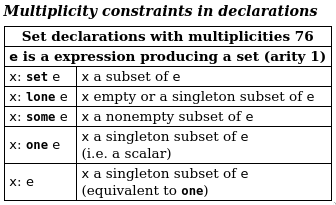
\includegraphics[width=0.4\linewidth]{img/alloy_multiplicity.png}
    \caption{Alloy Multiplicity constraints. Extracted from \cite{alloy-qr}.} 
    \label{fig:alloy-multiplicity}
\end{figure}


Structural constraints can be entailed over explicitly signature declaration. These are often referred as \textit{signature facts}, universally quantified over the signature's set \cite{alloy-qr}. Suppose a hypothetical design scenario, where the relation \textit{adj} is labelled as mutable. To ensure that the graph architecture consistency, in which, edges are structurally fixed, the following constraint can be specified. Additionally, consider the following \textit{graph} property, where it is desirable to express the following axiom: \textit{The graph contains no self-loops.}

\begin{lstlisting}[title={\textit{Node} hypothetical constraints over the signature definition.}, otherkeywords = {abstract, sig, module, var, set, fact, extends, no, in, this, not, always, \', \=}, floatplacement=H]
sig Node {
    var adj : set Node, 
    var visited : set Node
} {
    always adj' = adj
    this not in adj
}
\end{lstlisting}

As stated, the former poses a model incoherence within the \textit{Node} signature declaration, as \textit{adj} field is formerly labelled as mutable, that is later refuted by specifying $always \ adj'\ =\ adj$. This latter introduces the Alloy language's ability to express temporal behaviour through these \textit{two} \textit{linear temporal logic} operators, $'$ and $always$ respectively. 

\begin{figure}[H]
    \centering
    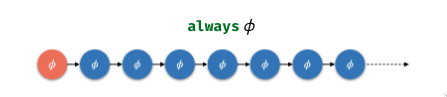
\includegraphics[width=0.7\linewidth]{img/alloy_always.png}
    \caption{$always$ behavioural representation.}
    \label{fig:alloy-always}
\end{figure}

The $always$ operator expresses a universal quantifier over time, imposing a constraint throughout the trace. The $'$ operator evaluates the \textit{adj} relation in the next state. So, the formula specifies that the evaluation of \textit{adj} in the next state is always the same of the current state. Alloy integrates LTL into the standard Relational logic, therefore, supporting both linear temporal logic unary and binary modal operator.

Whereas the latter expresses the \textit{no self-loop} graph property. Even though \textit{adj} is introduced as a relation between \textit{Nodes}, it is perceived as a set of \textit{Nodes} due to specification with the signature declaration. The keyword $this$ addresses each \textit{Node} atom, as self representation of the considered atom. The remaining specifies the intended behaviour, as it specifies the non-inclusion ($not\ in$) over the set of its adjacent nodes.

% The considered property expressness has a high level of complexity attached, and can be easily simplified over \textit{this not in adj}, as they both hold the same value. However, for contextualization reasons, and to introduce to the reader multiple Alloy's operators, the above is taken into account.

Aside from the structural constraints implied within signature's declaration, multiplicity over fields \ref{fig:alloy-multiplicity} and signatures also narrows the model's universe. The field multiplicity operators could be used to limit the number of signature atoms. Despite this, signature multiplicity is frequently used to represent singleton $one\ sig$ sets.

\begin{lstlisting}[title={\textit{Node} signature hierarchy.}, otherkeywords = {one, abstract, sig, module, var, set, fact, extends, no, in}, floatplacement=H]
one sig Init extends Node {}
var one sig Euler in Node {}
\end{lstlisting}

The above signatures accurately support the \textit{Eurelian} circuit concept. An \textit{Eurelian} path denotes a trail in a finite graph where every edge is visited exactly once. Additionally, an \textit{Eurelian} circuit implies that the path must start and end at the same node, denoted as \textit{Init}. As this latter differs from the remaining \textit{Node} atoms, the $extends$ keyword must be used to imply hierarchy disjointness. The \textit{Euler} node is an abstract representation of the current node that is being visited. As this impose a mutable state ($var$) over nodes, hierarchy disjointness is not appropriate. Hence, to properly model that the \textit{Euler} node can be included in an arbitrary atom, signature inclusion ($in$) should be used.

Both signatures are preceded by the $one$ keyword, imposing a multiplicity constraint over each signature declaration. Setting the multiplicity to $one$ means that each assessed model instance must have precisely one \textit{Init} atom and one \textit{Euler} atom. It should be noted that, since the \textit{Node} declaration is not preceded by the $abstract$ keyword, its atoms do not solely belong to the \textit{Init} signature. 

Additional modelling constraints can be specified by making use of the $fact$ declaration. The formula specified inside each $fact$ declaration denotes a model axiom, that holds a truth model assumption, to serve as a premise for further reasoning. 

The \textit{Eulerian} path denotes a trail within a finite graph, with each graph edge being visited precisely once. Thus, this already implies that the graph must be connected, where each node must be reachable, and undirected, where edges are non-oriented.

\begin{lstlisting}[title={Graph restrictions through $fact$ declaration.}, otherkeywords = {abstract, sig, module, set, fact, iden, no, in, \=, \*, \+, \~, \-\>, \&}, floatplacement=H]
fact eulerian_considerations {
    adj = ~adj
    no iden & adj
    Node->Node in *(adj + ~adj)
}
\end{lstlisting}

These expressions, above specified, make use of some valued Alloy operators, consequently identified either as a set-theory operator or as a relational operator. Despite the extensive number of operators supplied by Alloy's language, every expression, through the usage of \textit{FOL} quantifiers and \textit{LTL} operators, is later translated to boolean-based expressions. 

\begin{figure}[H]
    \centering
    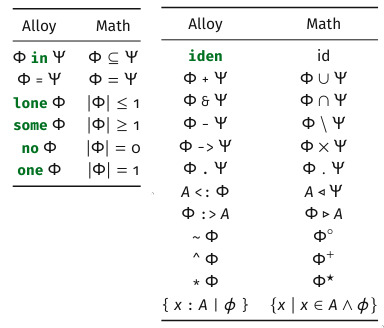
\includegraphics[width=0.5\linewidth]{img/alloy_relational_logic.jpg}
    \caption{Relational Logic Syntax.}
    \label{fig:alloy-rel}
\end{figure}

Regarding set-theory, set intersection (denoted by $\&$) and set conjunction (denoted by $+$) are introduced. The remaining are relational based operators. The $\sim adj$ denotes the converse relation of \textit{adj}, and the $\rightarrow$ represents the Cartesian product operator. The reflexive transitive closure operator ($\ast$) confers the
smallest transitive $\ast(adj\ +\ ~adj)$ relation containing all the identifiers, reachable in zero or more steps, through the implicit use of the set composition operator ($\cdot$). The other transitive closure $\string^$ is defined as $\string^ rel\ =\ \ast rel\ -\ iden$.

\begin{figure}[H]
    \[\string^ rel\ =\ rel\ + rel \cdot rel\ +\ rel \cdot rel \cdot rel\ + ... \]  
\caption{Reflexive transitive closure operator.}
\label{math:alloy-transitive}
\end{figure}

\subsubsection{Everything is a Relation}

As previously stated, Alloy emphasizes the mathematical relation concept to describe systems as a conventional designed model, through conceiving a set $R$ of relations. Moreover, Alloy confers the ability to express their relations as \textit{variable} \cite{lwspecification}. An Alloy relation presents itself as a set of tuples of \textit{atoms} drawn from the same universe context. Subsequently, each relation tuple must meet the same arity of the relation \cite{alloy-docs}.

The \textit{Alloy Evaluator} \cite{alloy-6} confers additional functionality to the \textit{Visualizer}. It allows the user to type Alloy-based expressions against the existing model, used to gather structure information about the existing model \cite{alloy-docs}. In the Figure \ref{fig:alloy-evaluator_1} is presented both \textit{Node} signature and \textit{adj} relation, regarding the model depicted in the Figure \ref{fig:alloy-eulerian_1}.

\begin{figure}[H]
    \centering
    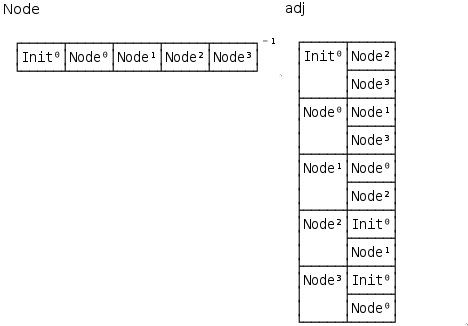
\includegraphics[width=0.5\linewidth]{img/alloy_evaluator1.png}
    \caption{\textit{Node} and \textit{adj} relations.}
    \label{fig:alloy-evaluator_1}
\end{figure}

Additionally, the use of the relational based operators $<:$ and $:>$ denote explicit restriction over relations, with the former restricting its domain, and the latter restricting its range.

\begin{figure}[H]
    \centering
    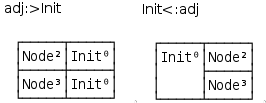
\includegraphics[width=0.4\linewidth]{img/alloy_evaluator2.png}
    \caption{\textit{Init} adjacent nodes.}
    \label{fig:alloy-evaluator_2}
\end{figure}


In order to prevent unwanted model structural scenarios, the intended model can be visualized over the \textit{Alloy Visualizer}, upon executing the $run$ analyzing command. In the Figure \ref{fig:alloy-eulerian_1} is depicted an instance of an acceptable configuration of the \textit{Eulerian} circuit with \textit{5 Node} atoms, since every model constraint was duly specified.

\begin{figure}[H]
    \centering
    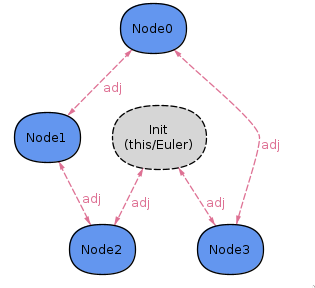
\includegraphics[width=0.5\linewidth]{img/alloy_eulerian_1.png}
    \caption{Acceptable \textit{Eulerian} graph model design.}
    \label{fig:alloy-eulerian_1}
\end{figure}



\subsection{Structural Behaviour}

Model's behaviour representation represents the ability to express what is intended to happen during state transitions over the valid traces of a system. A \textit{trace} is represented as an infinite chain of states that completely describes a system's potential behaviour. Valid traces are constrained by explicit specification of axioms, identified using the $fact$ keyword, alongside with the explicit model assumptions covered by each $sig$ declaration, also constrains the system's behaviour \cite{gheyi2007formally}.

Despite the usefulness in restricting the system's traces, it is not ideal to express every property as a model assumption. Alloy high level of expressiveness enables the behaviour representation over multiple forms through an event idiom \cite{lwspecification}.

System transitions are declared over events, where each event is conveniently specified in separate \textit{predicates}. The latter, denoted as $pred$, enables Alloy to express boolean formulas that only hold their value when invoked. 

Generally, events are specified with their respective event \textit{guards} and event \textit{effects}. A guard specifies a formula that must be true prior to the occurrence of the related event. Oppositely, an effect regards how the system evolves through the next state, providing a valid outcome of its event. The effect must account the mutable variables of the model through the usage of the $'$ operator, to guarantee the non-occurrence of unexpected behaviour. In addition, the temporal operator $after$ can be used to hold the truth of a formula in the next state.

\begin{figure}[H]
    \centering
    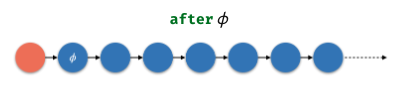
\includegraphics[width=0.6\linewidth]{img/alloy_after.png}
    \caption{$after$ behavioural representation.}
    \label{fig:alloy-after}
\end{figure}

In order to provide a proper contextualization over these concepts, it is desirable to recall the \textit{Eulerian} circuit example. The process of visiting nodes must be specified as it confers the main functionality within the graph theory. It follows the \textit{traverse} predicate to effectively express the latter process. 

\begin{lstlisting}[title={\textit{Eulerian} visiting event.}, otherkeywords = {pred, some, \:, \., not, in, ', \=, \+, \-\>}, floatplacement=H]
pred traverse {
    some adjn : Euler.adj {
        adjn not in Euler.visited
        visited' = visited + Euler->adjn + adjn->Euler
        Euler' = adjn
    }
}
\end{lstlisting}

The first guard states the existence of some node \textit{adjn}, that must be related to the \textit{Euler} node ($Euler \cdot adj$). Another guard is specified to cover the \textit{Eulerian} condition where each edge must be visited exactly once ($adjn\ not\ in\ Euler \cdot visited$). It is followed by \textit{2} effects, where the \textit{visited} relation must account the latest visited edge, and the \textit{Euler} node must be incorporated in the respective adjacent node, within the next state.

\begin{lstlisting}[title={\textit{Eulerian} stutter event.}, otherkeywords = {pred, ', \=}, floatplacement=H]
pred stutter {
    visited' = visited
    Euler' = Euler
}
\end{lstlisting}

Unexpected behavior can occur if no constraints are set on how the system grows through such mutable expressions. Constraints imposed on mutable expressions that should remain unchanged in the next state are referred as \textit{frame conditions}, a formula with primes ($'$) stating the "no change" effect \cite{alloy-docs}.

It is advisable to consider the "nothing changes" possibility in the evaluation of the trace evolution. The \textit{stutter} predicate captures the "no effect" reasoning approach about the behaviour of the system, where frame conditions formulas are enclosed between braces.

Every conceivable trace inside the system must be a permutation of these event handlers performed on a well-defined initial state. When used consistently, this approach constitutes a model design pattern called as Implicit Operation Idiom \cite{gheyi2007formally}.

\begin{lstlisting}[title={\textit{Eulerian} Initial State.}, otherkeywords = {pred, ', \=, no}, floatplacement=H]
pred _init {
    Euler = Init
    no visited
}
\end{lstlisting}

The \textit{\_init} states valid conditions valid in the first state. Thus, to properly specify the initial behaviour of our intended model, every edge must start unvisited ($no\ visited$) and the \textit{Euler} node should start in the \textit{Init} node.

As previously claimed, to reason about state transition, the notion of an execution trace should be duly introduced. The system's permissible behavior will be thoroughly specified by restricting the set of valid operations. As it already been specified every acceptable operation, it is presented the following $fact$ axiom. 

\begin{lstlisting}[title={Trace constraint through the use of an axiom.}, otherkeywords = {fact, ', \=, no, eventually, in\ , and, always, or}, floatplacement=H]
fact traces {
    _init
    always (move or stutter)
}
\end{lstlisting}

The temporal operator $always$ followed by the desired formula is used to impose a state constraint, that must hold one of the \textit{2} events, over the full trace evaluation. This axiom, as explained, must account the initial state (\textit{\_init}) conditions.

The notion of reusable expressions ($fun$) and model assertions ($assert$), are also conceptually included in the Alloy's event idiom. This idiom flexibility allows the developer to define action hierarchy, alongside with sharing atoms passed as parameters, resulting in simpler way of managing specifications \cite{lwspecification, alloy-docs}.


\section{Structural Analysis}

Structural modelling only confers a conventional way of formally expressing the intended behaviour over a software component. To perform verification over the specified behaviour, it is advisable to implement analysis techniques, while supporting an illustrative way of exploring the behaviour through simulations. 

Following the temporal logic semantics, Alloy specification language embeds the linear temporal logic into the first-order logic, thus, it makes use of both temporal and relational quantifiers to properly express behavioural verification over time \cite{lwspecification}. \textit{First-Order Temporal Logics} present additional techniques for reasoning about behaviour, while accounting the basis of the first-order logic, that usually confers the capability to express the well-formedness of the system structure \cite{lwspecification, konur2010survey}.

This section aims to explain how Alloy conducts system analysis, with further explanations over the corresponding analysis commands, along with an overview on the Alloy Analyzer interactive exploration over a system's design. 

\subsection{Analysis and Verification}

Alloy specification process does not establish a clear process separation over the model design and model analysis. This implies that analysis over model checking also accounts the model itself as a combination of properties specification. 

The specification language holds \textit{two} analyzing commands, $run$ and $check$ respectively, as shown above in \textit{Alloy's syntax}. A \textit{First-Order Linear Temporal Logic} (FOLTL) formula is enclosed between braces, to be checked over. Upon executing, both commands accounts the enclosed formula $\psi_{f}$ and the model declaration ${M}$. Likewise in $fact$ declaration, several logic constraints can be combined into the formula $\psi_{f}$. Due to Alloy's implicit abstraction, both commands addresses the relational model specification as truth holder, with the latter being consisted by declarations over $fact$ and $sig$. 

Briefly speaking, $run$ instruct the model-checker to present an example that satisfies the considered formula $\psi_{f}$ over the model definition. This means that the following formula ($M \wedge \psi_{f}$) is expected to hold. The consistency of the \textit{facts} and \textit{signatures} is consequently verified since the model declaration $M$ is also considered. 

Alloy makes use of the $check$ command to perform automatic verification over an $assertion$ declaration. The assertion $\psi_{f}$ verification is done over proving if the following satisfiability formula $M \models \psi_{f}$ is valid within the defined scopes. % while it accounts the declared \textit{facts} as truth holders. 

As result of the first-order logic's undecidability problem, the consistency proofness over satisfiability formulas is not possible \cite{vakili2012temporal}. To ensure decidability, the Alloy Analyzer performs analysis over \textit{scopes}, assigned to each signature declaration. By default, if no scope is provided, the model-checker will account at most \textit{three} atoms for each signature, upon trying to provide an \textit{instance} that satisfies the former formula, consequently proving the behaviour specification (\textit{facts} considerations) consistency. Also, as scopes imposes a limit on the state space of an Alloy model, if no $run$ instance is returned, the formula can not be perceived as inconsistent, as scopes can not be properly set to satisfy the latter.

\begin{figure}[H]
    \centering
    
\includegraphics[width=0.4\linewidth]{img/check_alloy_1.png}
    \caption{FOLTL formula $\psi$ verification using \textit{check}, accounting the \textit{Bounded} model checking technique.}
    \label{fig:alloy-check-1}
\end{figure}

Being SAT-based \cite{lwspecification}, the Alloy Analyzer tries to search for a \textit{lasso trace} instance that satisfies the formula $M \models \psi_{f}$ over the \textit{check} command, it performs the latter refutation ($(M \wedge \neg \psi_{p})$ by applying \textit{De Morgan's laws}), yielding a counter-example if the latter is satisfied. This technique is called \textit{Proof by Refutation}: $M$ entails $\psi_{p}$, denoted by $M \models \psi_{f}$, \textit{if and only if} $(M \wedge \neg \psi_{p})$ is unsatisfiable, reducing validity to unsatisfiability.

\begin{figure}[H]
    \centering
    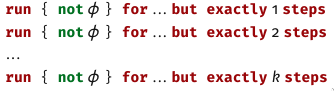
\includegraphics[width=0.5\linewidth]{img/check_alloy_2.png}
    \caption{Reducing Validity to Unsatisfiability.}
    \label{fig:alloy-check-2}
\end{figure}

Moreover, Alloy yields a command to specify the finite number of different steps, related to the expected instance's evaluation trace. This is due to the bounded nature of the Alloy transitions between states, where the \textit{Bounded Model Checking} is considered as model-checking technique. The number of steps is set to \textit{10} by default, although this may be adjusted using the keyword $steps$, alongside with the bounded scopes specification. 

The following $run$ example makes use of both scopes and steps definitions. Moreover, the formula specified in the $run$ states the expected behavioural representation of an \textit{Eulerian} circuit. The $eventually$ (Figure \ref{fig:alloy-eventually}) operator is considered to specify the desired final state, where every edge is visited and the \textit{Euler} node finishes where it started.

\begin{lstlisting}[title={Bounded Model Checking: Eventually the graph will represent an \textit{Eulerian} circuit.}, otherkeywords = {run, eventually, in, and, for, exactly, \5, steps}, floatplacement=H]
run example {
    eventually (adj in visited and Euler in Init)
} for exactly 5 Node, exactly 5 steps
\end{lstlisting}

This particular $run$ yields no instance, so its corresponding formula $M \wedge \psi_{p}$ does not hold, since imposing \textit{5} steps is not sufficient to provide an instance where the desired state, defined by the latter formula, is reached.


\subsubsection{Behavioural Properties}

The verification process over \textit{Model Checking}, needs to account the formal specification of properties that are relevant to reason about the system's temporal behaviour \cite{baier2008principles} .

Alloy makes use of the relational logic (Figure \ref{fig:alloy-rel}) to ensure the well-formedness of the system, which falls short when it comes to supplying support over temporal behaviour. Thereby, Alloy includes temporal connectives from FOLTL semantics, that acknowledges the system's states along the trace evolution \cite{lwspecification, alloy-6, 9341085}.

Ensuring the correctness of a system's behaviour relies on verifying properties regarding the latter's \textit{Safety} and \textit{Liveness}. Its verification technique is motivated by distinct approaches \cite{kindler1994safety}. The former requires an invariance argument, where the latter requires a well-foundedness argument to prove its system satisfiability \cite{alpern1987recognizing}.

A \textit{safety property} asserts that "nothing bad should happen" during the system execution, meaning that, every trace state is expected. Consequently, if a trace that jeopardizes a safety property is found, it can be assumed that the latter has a "bad" property prefix. 

\begin{lstlisting}[title={\textit{Safety Property}: The relation visited can only evolve through time.}, otherkeywords = {always, assert, module, set, fact, iden, no, in, \=, \*, \+, \~, \-\>, \&, '}, floatplacement=H]
assert safety_visited {
    always visited in visited'
} 
\end{lstlisting}

\begin{lstlisting}[title={\textit{Safety Property}: If a node is visited, then once \textit{Euler} was 'inside' it.}, otherkeywords = {always, assert, module, set, fact, iden, no, in, \=, \*, \+, \~, \-\>, \&, all, \:, \., implies, once}, floatplacement=H]
assert safety_euler {
    always (all n :  Node | n in Node.visited implies once Euler = n)
} 
\end{lstlisting}

\begin{figure}[H]
    \centering
    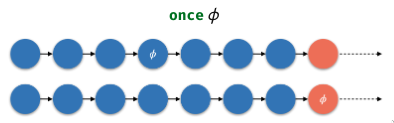
\includegraphics[width=0.6\linewidth]{img/alloy_once.png}
    \caption{$once$ behavioural representation.}
    \label{fig:alloy-once}
\end{figure}

Whereas, a \textit{liveness property} expresses that "something good will happen", implying the eventual occurrence of a state during the course of the system's execution \cite{lamport1977proving}.

\begin{lstlisting}[title={\textit{Liveness Property}: Eventually the graph will represent an \textit{Eulerian} circuit.}, otherkeywords = {assert, eventually, in, and}]
assert liveness_euler {
    eventually (adj in visited and Euler in Init)
} 
\end{lstlisting}

\begin{figure}[H]
    \centering
    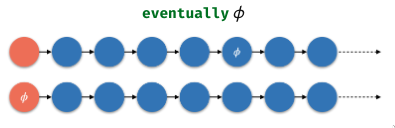
\includegraphics[width=0.6\linewidth]{img/alloy_eventually.png}
    \caption{$eventually$ behavioural representation.}
    \label{fig:alloy-eventually}
\end{figure}

The above-mentioned properties make use of \textit{2} relevant over time quantifiers. The $once$ operator expresses the past validation of a given formula. The $eventually$ operator expresses an existence quantifier, imposing the formula verification somewhere along the trace evolution \cite{alloy-docs}.

Moreover, the liveness property states the expected behavioural representation of an \textit{Eulerian} circuit, where the $eventually$ (Figure \ref{fig:alloy-eventually}) operator is considered to specify the desired final state. However, its verification, using $check\ liveness\_euler$, yields a counterexample, as it is possible to always perform the \textit{stutter} event, and thus the expected behaviour never happens. This scenario results in an implausible infinite trace behavior, which must be handled by adding fairness to the trace assessment. 

Liveness properties evaluation process reasons about states that eventually might reach the wanted scenario. Then, it is advisable to consider \textit{fairness} constraints, intentionally specified to rule out infinite traces with unrealistic behaviour, such as system stuttering \cite{baier2008principles}. Briefly, a \textit{fairness} constraint imposes fairly considerations on the system's trace evolution \cite{wahlfairness}.

\begin{lstlisting}[title={\textit{Fairness predicate}: If \textit{Euler} has an adjacent node, it will eventually visit the latter.}, otherkeywords = {pred, eventually, always, implies, some, \.}]
pred fairness {
	(eventually always some Euler.adj) implies (always eventually traverse)
}
\end{lstlisting}

The latter imposes a fairness constraint regarding the trace evolution, ensuring that trace stuttering is not possible as long as the \textit{Euler} node has some adjacent node that is not been visited yet. As expected, by instructing the Analyzer to check the asserted property ($check\ liveness\_euler$), it will return no counterexample.

\begin{lstlisting}[title={\textit{Liveness} property accounting the fairness constraint. It yields no counterexample.}, otherkeywords = {assert, in, and, eventually, check}]
assert liveness_euler {
	fairness implies eventually (adj in visited and Euler in Init)
} check liveness_euler
\end{lstlisting}

\subsection{Alloy Analyzer}

Normally, the specification process upon abstracting the system as a conventional model is carried out interactively, since considerations about model validation must be preceded by the model specification. The already mentioned analysis techniques, $run$ and $check$ analysis commands respectively, instruct the Analyzer to check and provide analysis over their implicit formula nature. 

Moreover, the Analyzer is capable of providing model instances concerning the formula evaluation, depicted graphically as graph-like structures, through the usage of the Alloy \textit{Visualizer}. The latter allows instance interaction over multiple configuration buttons. Additionally, concerning the user comprehension, the graphical depiction of these instances can be customized using \textit{Themes}, through the \mybox{Theme} toolbar button.

Recall the $run$ example that failed to provide a model instance due to the $steps$ explicit limitation. To find an \textit{Eulerian} circuit instance for $n$ nodes, the minimum of $n+1$ steps are required.

\begin{lstlisting}[title={Bounded Model Checking: Eventually the graph will represent an \textit{Eulerian} circuit.}, otherkeywords = {run, eventually, in, and, for, exactly, \5, steps}, floatplacement=H]
run example {
    eventually (adj in visited and Euler in Init)
} for exactly 5 Node
\end{lstlisting}

Producing a concrete instance might be quite helpful throughout the modeling process. The $run$ command presented above is capable of providing a model instance as it performs Bounded Model Checking for at most \textit{10} steps. The Analyzer executes the command and generates an instance regarding the latter, consequently producing a visual graphical (Figure \ref{fig:alloy-valid-run}) through the usage of the Visualizer.

\begin{figure}[H]
    \centering
    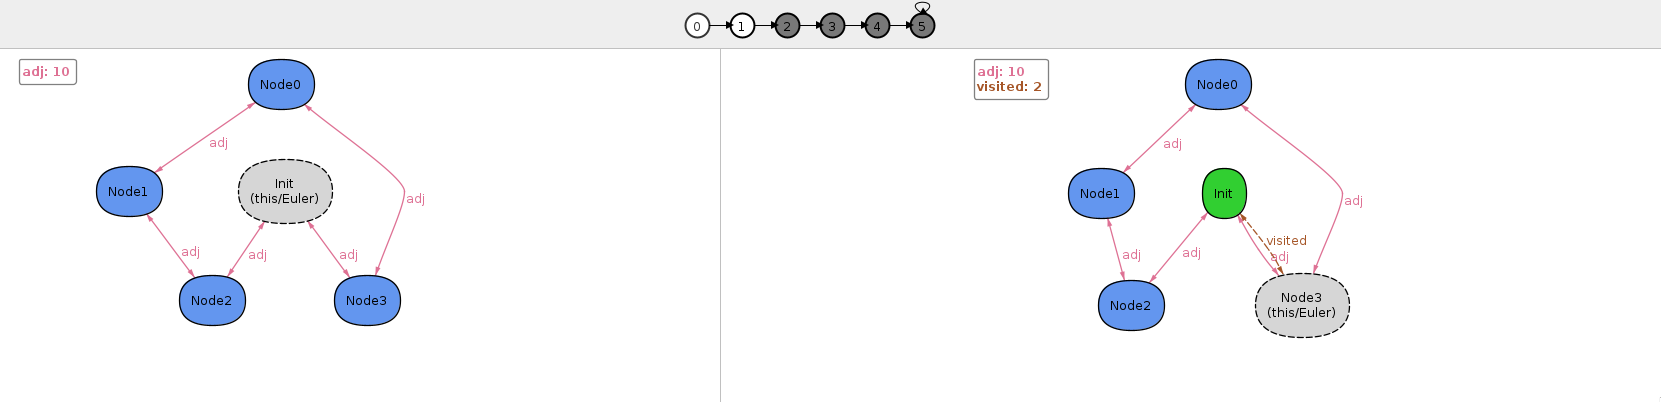
\includegraphics[width=\linewidth]{img/alloy_run.png}
    \caption{Partial graphical view of the \textit{two} initial states. The \textit{Euler} node starts in the \textit{Init} node, and then moves towards an adjacent node.}
    \label{fig:alloy-valid-run}
\end{figure}

The Visualizer furnishes a toolbar with multiple configuration buttons, allowing interactive customization over alternative instances \cite{alloy-docs}. Traces can also be interactively overviewed through transition buttons ($ \rightarrow $ and $ \leftarrow $), enabling forward and backward trace navigation.

\begin{figure}[H]
    \centering
    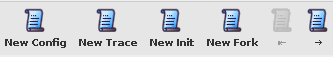
\includegraphics[width=0.7\linewidth]{img/alloy_buttons.png}
    \caption{Alloy Visualizer toolbar.}
    \label{fig:alloy-toolbar}
\end{figure}

The \mybox{New Config} instructs the Analyzer to provide a new trace configuration, where immutable model expressions (sets and relations) are depicted with new values. Consequently, the Visualizer will present an execution trace regarding the new model configuration. The \mybox{New Trace} instructs the Analyzer to present a new execution trace, regarding the same model configuration. The \mybox{New Init} requests for a new trace representation, where the initial state is forced to present different model expressions values. At last, the \mybox{New Fork} allows alternative transition behaviour exploration over the same starting state, depicting a new transition post-state. The latter could differ on the result of a given event, or it can display the outcome of a different event \cite{alloy-docs}.

Alloy forces the property formula translation into an LTL-based formula, considering the finitude of its universe of comprehension. Due to the emphasis on representing instances over infinite traces, every Alloy instance generated by the Analyzer, captures an infinite trace through \textit{lassos}, where a looping state is reached.

Concerning performance in the evaluation over infinite traces, Alloy considers the Bounded Model Checking technique as the first approach towards the model verification. Here, the corresponding formula is verified for all \textit{lasso} traces of size up to a bounded number of steps. So, the verification is not complete, due to the SAT time-bounded nature. However, it still confers great functionality, as infinite traces can often be represented as finite traces, making verification within small scopes possible \cite{jackson2012software}.

\begin{figure}[H]
    \centering
    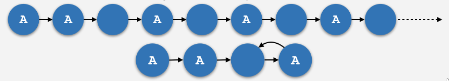
\includegraphics[width=0.7\linewidth]{img/alloy_infinite_trace.png}
    \caption{Some infinite traces can be represented by finite \textit{lasso} traces.}
    \label{fig:alloy-infinite}
\end{figure}

Oppositely, the Analyzer can be instructed to perform \textit{Unbounded Model Checking} towards achieving consistency over model verification, without bounding traces upfront \cite{alloy-6, alloy-docs}. This is feasible as the state space is finite due to the Alloy analysis way of bounding signatures. Consequently, it constrains infinite traces as periodic \textit{lasso} traces (Figure \ref{fig:alloy-infinite}).

To perform complete model-checking, an appropriate solver must be selected in the \mybox{Options} menu, and the time scope must be specified under the following syntax: $for\ 1..\ steps$. Consider the previous $run$ command in terms of the Unbounded Model Checking approach. 

\begin{lstlisting}[title={Unbounded Model Checking: Eventually the graph will represent an \textit{Eulerian} circuit.}, otherkeywords = {run, eventually, in, and, for, exactly, \5, steps}, floatplacement=H]
run example {
    eventually (adj in visited and Euler in Init)
} for exactly 5 Node, 1.. steps
\end{lstlisting}

\section{Related Work}\label{s:relWork-pv}

As reliance on robotic systems grows due to their expanding application across a wide range of domains, these systems concern critical scenarios, where human interaction comes in hand \cite{diluoffo2018robot}. Thus, security should be highly considered upon employing systems that might jeopardize the human's integrity, such as robotics. Additionally, ensuring analysis regarding the system's quality assurance is increasingly becoming a focus of attention. Consequently, it is critical to employ techniques that promote the increase of the system quality, without sacrificing its flexible nature.

\citeauthor{cortesi2013static} in \textit{Static Analysis Techniques
for Robotics Software Verification} \cite{cortesi2013static} gives a proper understanding on how important it is to perform formal analysis to ensure  the reliability of the resulting software, while significantly minimizing the testing effort. Here, the authors intend to cover multiple static analysis techniques to properly contextualize robotic developers about which is the most appropriate analysis strategy to follow based on the kind of examined property and software system. After briefly introducing to each technique, the authors present an overall evaluation of the various static analyzes techniques, following several criteria: automation, precision, scalability, and soundness. \citeauthor*{cortesi2013static} conclude stating that performing analysis techniques is highly fundamental to develop robotics software. Additionally, the authors discuss the difficulties of guaranteeing adequate automated analysis of complex properties. Finally, they emphasize the need of future reasearch within this formal verification context, due to its role in software development. 

This section concerns the study of some relevant studies that introduces to some pertinent quality assurance procedures over the robotics domain. The latter's concentration will be on the following subjects: First, system analysis regarding static procedures will be contextualized, emphasizing a notable framework, called \textit{HAROS}, that performs static evaluation over ROS-based applications; After that, various state-of-art methodologies based on property verification are given as support to this dissertation analysis approach.

Even though this dissertation was devoted to a detailed examination of ROS framework regarding its security deployment, there is no obvious line separating the ROS difficulties from those of other popular multi-configurable robotic software in terms of quality assurance and security overview. As result, a broader range of robotic systems will be explored to give contextualization of some relevant aspects that also fall under the ROS domain.

Analysis through property verification in the ROS framework represents a major contribution to this dissertation domain, in which researchers aim to tackle issues arose from miss configurations or code inconsistencies. Although researches and tools on analysis of ROS systems are scarce, there are some presented work that might be useful within the context of this dissertation.

For instance, a natural way of performing analysis over a system is by observing the communication architecture. Recall that the Alloy Visualizer is useful to observe the system behaviour as traces through state evaluation. Here, ROS provides a framework for GUI development plugin called \textit{rqt\_graph} \footnote[2]{http://wiki.ros.org/rqt\_graph}, in which ROS developers usually rely on. It is used to depict the network architecture through a graph with run-time statistics. However, this approach lacks on providing trustworthy analysis over more complex networks, where features such as security control are implicit.

The noteworthy \textit{HAROS} framework, initially proposed by \citeauthor{santos2016framework} in \textit{A framework for quality assessment of ROS repositories} \cite{santos2016framework}, holds great value thanks to its contribution in improving ROS's software quality. \textit{HAROS} makes use of several analysis techniques to exert quality evaluation of ROS software, followed by ways of feed-backing inconsistencies using predefined code metrics. As this framework seeks to be flexible when it comes to adding functionality, further static analysis works improvements have been proposed as plugins.

In both \citenum{santos2019static} and \citenum{santos2018property}, it is presented additional functionality to the framework, through applying architectural considerations over metamodel designing, where the latter supports the former by supplying property-based specifications. These techniques confers great help back to developers, since static analysis offers advantageable usage over raw review of software code. 

The literature concerning property verification has already been explored through state-of-art model checkers, where safety properties regarding the robotics domain were studied and verified. Within the ROS context, certain techniques were proposed that primarily focused on modeling the ROS node-communication, while real-time properties were also considered as support to the target language.
 
Within this context, \citeauthor*{halder2017formal} provides a model-based approach to reason about the communication between nodes in ROS-based systems, emphasizing the specification of real time properties. Here, the authors apply model techniques over ROS applications, abstracting them as timed automatas. Property verification is then ensured by model checking through the \textit{UPPAAL} \footnote[3]{https://uppaal.org/} model checker. 

Notably, this work provides a brief introduction to the concepts of timed automata and their implementation into \textit{UPPAAL}, with respect to the latter's temporal logic as a query language to describe desired properties. After contextualizing the code behind a ROS-based application, the authors proceed to perform model checking using the source code of a popular physical robot \textit{Kobuki} \footnote[4]{http://kobuki.yujinrobot.com/}. This allowed the authors to reason about context specific properties of the latter, aside from the safety properties.

\citeauthor*{halder2017formal} conclude their work by emphasizing the importance of model-checking in finding and checking these desirable properties, stating if only physical verification was considered, the latter's properties would be extremely difficult, time-consuming or infeasible to find.

A noteworthy study is supplemented by \citeauthor*{white2019network}, in \textit{Network Reconnaissance and Vulnerability Excavation of Secure DDS Systems} \cite{white2019network}. \citeauthor{white2019network} continues to address security \cite{white2016sros, white2018procedurally} through an alternative approach. Here, the author makes use of formal verification and model checking to reason about reachability of information flow, related to an attack model that studies the network through targeted attacks. This study starts to overview the DDS security protocol and its model, to make further speculations about the lack of support for some additional security threats from the latter. 

Within this scenario, \citeauthor{white2019network} intends to explore the data flow semantics to address the DDS networks vulnerability. After conceiving the threat model, some attack assumptions are explicitly defined over the attack model. Unlike previous network reconnaissance methods and considering the assumptions discussed in the attack model, this approach allows an attacker to build the topology through a graph based database by passively sniffing packets inside the network. This database is then made available to the SAT solver in order for it to compute queries. \textit{Imandra} \footnote[5]{https://www.imandra.ai/} model checking tool is then used as SAT solver by replicating the DDS security protocol functionalities (especially the access control) as functional models, to accurately represent default plugin logic. Thus, the attack model assumptions can be then specified over SAT queries, allowing the replicated models to reflect a new SAT. Moreover, using formal verification and model checking, vulnerability excavation can be efficiently performed over the inquired graph, instead of engaging with the targeted system. 

The authors conclude their work by reasoning about how crucial is to employ attack models for general system validation. Also, the usage of formal verification techniques can reason about a large state space without exhaustive search.

A remarkable work that duly fits under this dissertation domain of exploration is presented in \citenum{9341085}. Here, \citeauthor{9341085} presents a notable proposal to automatically verify system-wide properties of ROS applications at static time, emphasizing their safeness behaviour. Here, the authors intend to abstract each application behaviour through concrete models, to then perform model-checking over system-wide specifications, using \textit{Electrum} as model checker. 

In order to integrate analysis of ROS-based applications, the authors make use of the already mentioned \textit{HAROS} plugin-based framework, that provides quality assessment of ROS software. \textit{HAROS} allows the automatic extraction of the system structure based-on an architectural model, based on a static analysis of the source code. Then, using a domain-specific property-based language, it allows reasoning about the specialist's system behavior. 

\begin{figure}[H]
    \centering
    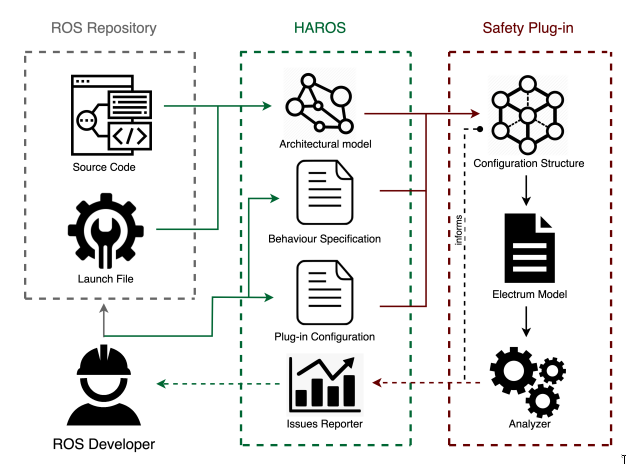
\includegraphics[width=0.6\linewidth]{img/haros-electrum-plugin.png}
    \caption{Architecture of the \textit{HAROS} safety plugin for ROS. Extracted from \cite{9341085}.}
    \label{fig:haros-electrum}
\end{figure}

The safety plugin denotes the backend of the depicted architecture (Figure \ref{fig:haros-electrum}), where it relies on \textit{Electrum}, the former version of the current \textit{Alloy Analyzer}, to model and reason about the application behaviour through properties expressed in FOTL. Afterwards, the authors pretend to extend \textit{HAROS}' functionality by offering a plugin that automatically converts \textit{HAROS} artifacts into \textit{Electrum}. Additionally, the framework reports model checking counter-examples in a more user-friendly manner via its quality reporting interface. 


Through ROS launch configurations, the plugin automatically generated models using Electrum and performs verification over these models, to then feedback issues related to their ROS system behaviour.

As ROS2 domain regards the use of DDS communication protocol, a few works on DDS modelling analysis deserve to be mentioned, as they might give important background for property verification over communications protocols. In \citenum{alaerjan2017modeling}, it is proposed a technique to model the DCPS architectural design that DDS makes use of, alongside with new approaches to the current DDS behaviour. Supported by several modelling techniques for publish-subscribe systems, in \citenum{liu2018formal}, DDS in ROS2 is formalized as a timed automata, consequently followed by model verification over property-checking. These works conceive value concepts and procedures useful for this dissertation contextualization.

A few studies on robotics should be recognized in which techniques such as model-checking were performed. Despite the fact that they do not address the domain of ROS, they nonetheless give helpful background for the robotics research over formal approaches. 

A case study, mentioned in \citenum{near2011lightweight}, presents a novel approach over systems that require static analysis based on software assumptions and proper analysis within its environment usage, where user-interaction comes in hand. Concerning this novel idea, a medical system is concerned as a case study, where multiple safety-based considerations are expected, as well as, an end-to-end critical property that must be satisfied over the entire analysis course. 

Another notable work regarding former analysis using Alloy specification language is presented in \citenum{mansoor2018modeling}, where a safety-critical scenario is proposed under the domain of surgical robots. The formal techniques used allows overview over a surgical robot arm, taking into consideration possible violations of important safety properties. 

Although these studies presents favorable outcomes, their focus lies on a particular area of study. As a result, they lack on providing solutions to a vast majority of situations.

\chapter{Future Work}\label{c:currWork}

This chapter provides a brief introduction over the problems that this dissertation aims to tackle, supported by a graphical dissertation schedule, in which the main development tasks are organized over time.

Following the \textit{Literature review} period where background concepts were duly studied and the pre-dissertation was written, it is expected that within the next first month security-related discussions will take place as major priority, due to its critical role on what this dissertation aims to tackle. Properties regarding security will be properly supported by ROS examples. Thus, it is intended to find concrete example that fails to address a specific security property, where the latter would be previously evaluated in a speculative manner. 

Afterwards, the already discussed schedule and respective assigned timings can proceed its predefined order. Here, ROS2 applications architectures will be formalized in Alloy, where the above's considerations about security and SROS2 configuration specification will be taken into account upon the modelling process. Then, it is expected to propose  a technique to specify and verify information-flow security properties on top of the proposed Alloy formalization.

Both \textit{Evaluation} and \textit{Implementation} periods will follow the latter's objectives. After concluding the \textit{Implementation}, the dissertation writing and review will proceed in order to present the full work on paper.

\begin{figure}[H]
    \centering
    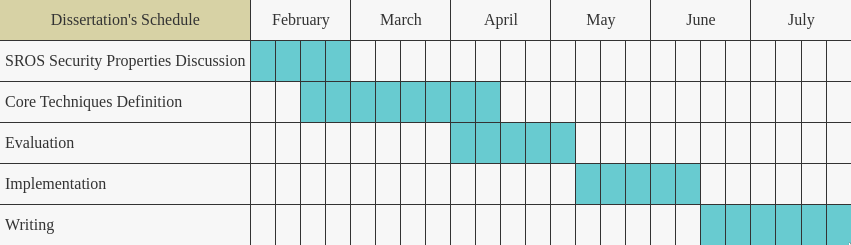
\includegraphics[width=\linewidth]{img/dissertation-schedule.png}
    \caption{Dissertation's schedule.}
    \label{fig:dissertation-schedule}
\end{figure}

The whole timetable is displayed above in the form of a table (Figure \ref{fig:dissertation-schedule}), with the times evenly split among the several periods. 
A more thorough schedule with related sub-tasks is shown below to completely contextualize the whole work that is planned to occur.

\begin{itemize}
\item SROS2-related Security Properties:
    \begin{itemize}
        \item Discussion and Overview.
    \end{itemize}

\item Core Techniques Definition:
    \begin{itemize}
        \item Formalization of the architecture of ROS2 applications in Alloy.
        \item Extend this formalization to cover the SROS2 security configuration.
        \item Propose a technique to specify and verify information-flow security properties on top of the proposed Alloy formalization.
    \end{itemize}

\item Evaluation:
    \begin{itemize}
        \item Selection of relevant case studies in the \textit{Autoware} platform.
        \item Identify and formalize relevant information-flow security properties for that case study.
        \item Evaluate the effectiveness of the proposed formalization and verification technique on the identified case studies and security properties.
    \end{itemize}

\item Implementation:
    \begin{itemize}
        \item Implement a prototype tool that can automatically infer an Alloy formalization of a ROS2 architecture and SROS2 security configuration.
    \end{itemize}

\item Writing:
    \begin{itemize}
        \item Finish dissertation writing.
        \item Dissertation review.
    \end{itemize}
\end{itemize}

%\chapter{Evaluation}\label{c:Evaluation}


%\chapter{Conclusion}\label{c:conc}

%Lá chegará o dia em que haverá algo para concluir.

%\section{Citations}
%Example of a citation: \cite{GRM97}, cf.\ this entry in the \Bibtex\ file.
%Another way of citing is \citep{KeR88}
%
%\chapter{The problem and its challenges}
%         The problem and its challenges.
%
%\section{Images}
%	Example of inserting an image as displyed text,
%\begin{center}
%	
\includegraphics[width=0.2\textwidth]{img/mei-logo-03.jpg}
%\end{center}
%
%\begin{wrapfigure}{r}{0.25\textwidth}
%	
\includegraphics[width=0.2\textwidth]{img/mei-logo-03.jpg}
%\end{wrapfigure}
%\noindent --- wrapped into the text,
%bla-bla bla-bla bla-bla bla-bla bla-bla bla-bla bla-bla bla-bla bla-bla bla-bla
%bla-bla bla-bla bla-bla bla-bla bla-bla bla-bla bla-bla bla-bla bla-bla bla-bla
%bla-bla bla-bla bla-bla bla-bla bla-bla bla-bla bla-bla bla-bla bla-bla bla-bla
%bla-bla bla-bla bla-bla bla-bla bla-bla bla-bla bla-bla bla-bla bla-bla bla-bla
%bla-bla bla-bla bla-bla bla-bla bla-bla bla-bla bla-bla bla-bla bla-bla bla-bla bla-bla bla-bla bla-bla bla-bla
%bla-bla bla-bla bla-bla bla-bla bla-bla bla-bla bla-bla bla-bla bla-bla bla-bla bla-bla bla-bla bla-bla bla-bla
%
%\noindent --- or as a floating body.
%\begin{figure}
%\begin{center}
%	
\includegraphics[width=0.5\textwidth]{img/mei-logo-03.jpg}
%\end{center}
%\caption{Caption}
%\end{figure}
%
%You can also use an image as an icon, eg.\ \MEI, in the main tex.
%Click on it to visit the website. It is also listed in the list of terms.
%Another example of an item to appear in the term index: \UM (needs \Makeindex)
%
%\begin{table}[]
%\begin{tabular}{lllll}
% &  &  &  &  \\
% &  &  &  &  \\
% &  &  &  &  \\
% &  &  &  &
%\end{tabular}
%\caption{Caption}
%\end{table}
%
%\part{Core of the dissertation}
%
%\chapter{Contribution}
%	Main result(s) and their scientific evidence
%\section{Introduction}
%\section{Summary}
%
%\chapter{Applications}
%	Application of main result (examples and case studies)
%\section{Introduction}
%\section{Summary}
%
%\chapter{Conclusions and future work}
%	Conclusions and future work.
%\section{Conclusions}
%\section{Prospect for future work}

\bookmarksetup{startatroot} % Ends last part.
\addtocontents{toc}{\bigskip} % Making the table of contents look good.
\cleardoublepage

%----------------- Bibliography (needs bibtex) --------------------------------%
\bibliography{dissertation}
%----------------- Index of terms (needs  makeindex) --------------------------%
\printindex
%------------------------------------------------------------------------------%

	\appendix
	\renewcommand\chaptername{Appendix}

	% Add appendix chapters

%\part{Appendices}
%
%\chapter{Support work}
%	Auxiliary results which are not main-stream
%
%\chapter{Details of results}
%         Details of results whose length would compromise readability of main text.
%
%\chapter{Listings}
%	Should this be the case

%\chapter{Tooling}
%	(Should this be the case)

%	Anyone using \Latex\ should consider having a look at \TUG,
%	the \tug{\TeX\ Users Group}

\begin{backcover}
\thispagestyle{empty} \pagecolor{white} \textcolor{black} {\fontfamily{phv}\fontseries{mc}\selectfont ~\vfill
\noindent
NB: place here information about funding, FCT project, etc in which the work is framed. Leave empty otherwise.
%
\vfill ~}
\end{backcover}

\end{document}

